\documentclass[a4paper]{article}

\usepackage[UTF8]{ctex}
\usepackage[a4paper,margin=1in]{geometry}
\usepackage{graphicx}
\usepackage{float}
\usepackage{listings}
\usepackage{longtable}
\usepackage{booktabs}
\usepackage{hyperref}
\usepackage{fancyhdr}
\usepackage{lastpage}
\usepackage{color}
\usepackage{indentfirst}        % 首段缩进
\setlength{\parindent}{2em}     % 缩进2字符
\usepackage{zhnumber}           % 中文编号
\usepackage[dvipsnames]{xcolor}
\usepackage{amsmath}            % 数学公式
\usepackage{subcaption}         % 子图排版

\newcommand{\college}{中山大学计算机学院}
\newcommand{\projname}{人工神经网络| Lab1}
\newcommand{\reporttitle}{从零手写神经网络}
\newcommand{\stuno}{23336179}
\newcommand{\authorname}{马福泉}
\newcommand{\major}{计算机科学与技术}
\newcommand{\adviser}{潘炎}
\newcommand{\startdate}{2026年5月1日}
\newcommand{\labenddate}{2026年5月12日}
\newcommand{\labroom}{B201}

\pagestyle{fancy} % 使用 fancyhdr 风格
\fancyhf{}      % 清空默认的页眉页脚

% 设置页眉
\fancyhead[L]{\kaishu \projname}      % 左侧页眉显示项目名称
\fancyhead[C]{\kaishu \reporttitle}    % 中间页眉显示报告标题
\fancyhead[R]{\kaishu \authorname} % 右侧页眉显示作者姓名

% 设置页脚
\fancyfoot[C]{第 \thepage 页，共 \pageref{LastPage} 页} % 中间页脚显示页码

% 去除页眉页脚与正文之间的分隔线
\renewcommand{\headrulewidth}{0.4pt}
\renewcommand{\footrulewidth}{0pt}

% 设置文档背景颜色
\definecolor{mybgcolor}{RGB}{0, 0, 0} % 定义背景颜色
\definecolor{NavyBlue}{RGB}{0,0,128} % 添加颜色定义

% listing 配置python（美观样式）
\definecolor{codegreen}{RGB}{0,128,0}
\definecolor{codegray}{RGB}{128,128,128}
\definecolor{codepurple}{RGB}{128,0,128}
\definecolor{codeblue}{RGB}{0,0,255}
\definecolor{codeorange}{RGB}{255,128,0}

\lstset{
    language=Python,
    basicstyle=\ttfamily\footnotesize,
    keywordstyle=\color{codeblue}\bfseries,
    commentstyle=\color{codegreen}\itshape,
    stringstyle=\color{codepurple},
    numbers=left,
    numberstyle=\tiny\color{codegray},
    stepnumber=1,
    numbersep=5pt,
    backgroundcolor=\color{white},
    showspaces=false,
    showstringspaces=false,
    showtabs=false,
    frame=single,
    tabsize=4,
    captionpos=b,
    breaklines=true,
    breakatwhitespace=false,
    escapeinside={(*@}{@*)},
    extendedchars=true,
    inputencoding=utf8,
    literate={：}{{：}}1 {（}{{（}}1 {）}{{）}}1,
    morekeywords={self, True, False, None, as, with, yield, lambda, assert, raise, except, finally, import, from, pandas, numpy, pd, np, sklearn, fit, predict, recommend, DataFrame, Series, defaultdict, cosine_similarity, TfidfVectorizer}
}

\begin{document}

% 封面
\begin{titlepage}
    \centering
    
    % 校徽
    
\includegraphics[width=0.8\textwidth]{img/SYSULogo.png}
    \vspace{1em}

    \vspace{1em}
    {\Large \kaishu \college \par}
    \vspace{1em}
    {\Large \kaishu \projname \par}
    \vspace{3em}

    
    {\fontsize{40pt}{42pt}\kaishu \selectfont \boldmath \reporttitle\par}
    \vspace*{\fill}

    \begin{center}
    {\Large
    \makebox[5em][s]{学号}:\underline{\makebox[15em][c]{\kaishu \stuno}}\\[1em]
    \makebox[5em][s]{姓名}:\underline{\makebox[15em][c]{\kaishu \authorname}}\\[1em]
    \makebox[5em][s]{专业}:\underline{\makebox[15em][c]{\kaishu \major}}\\[1em]
    \makebox[5em][s]{指导教师}:\underline{\makebox[15em][c]{\kaishu \adviser}}\\[1em]
    \makebox[5em][s]{起始日期}:\underline{\makebox[15em][c]{\kaishu \startdate}}\\[1em]
    \makebox[5em][s]{结束日期}:\underline{\makebox[15em][c]{\kaishu \labenddate}}\\[1em]
    \makebox[5em][s]{实验地点}:\underline{\makebox[15em][c]{\kaishu \labroom}}
    }
    \end{center}

    \vspace*{\fill}
\end{titlepage}

% 目录
\tableofcontents
\newpage

\section{实验简述}

\subsection{实验内容}

本次实验是人工神经网络课程的第一次大作业，要求使用纯 Python/NumPy 从零实现深度神经网络的核心组件，不允许使用 PyTorch、TensorFlow 等深度学习框架。实验内容涵盖以下五大模块：

\subsubsection{激活函数（8分）}

依照 \texttt{ActivationFunction.ipynb} 中的要求：
\begin{enumerate}
    \item 实现 sigmoid 激活函数的前向传播和反向传播（4分）
    \item 实现 tanh 激活函数的前向传播和反向传播（4分）
\end{enumerate}

\subsubsection{全连接神经网络（15分）}

依照 \texttt{FullyConnectedNets.ipynb} 中的要求：
\begin{enumerate}
    \item 实现 affine layer 的前向传播和反向传播（3分）
    \item 实现 ReLU 激活函数的前向传播和反向传播，并在 Jupyter Notebook 上回答问题 1（3分）
    \item 利用实现的 affine layer 和 ReLU 激活函数构建一个两层的全连接神经网络（3分）
    \item 训练实现的两层全连接神经网络，使测试结果的准确率达到 50\% 以上（3分）
    \item 构建多层的全连接网络，满足 \texttt{FullyConnectedNets.ipynb} 中的测试要求（3分）
\end{enumerate}

\subsubsection{归一化（10分）}

依照 \texttt{BatchNormalization.ipynb} 中的要求：
\begin{enumerate}
    \item 实现 batch normalization 的前向传播和反向传播（3分）
    \item 修改之前实现的全连接神经网络，添加 batch normalization，回答问题 1（3分）
    \item 探究 batch normalization 和 batch size 的关系，回答问题 2（2分）
    \item 实现 layer normalization 的前向传播和反向传播，并将 layer normalization 添加到之前实现的全连接神经网络中（1分）
    \item 探究 layer normalization 和 batch size 的关系，回答问题 3（1分）
\end{enumerate}

\subsubsection{CNN（32分）}

依照 \texttt{ConvolutionalNetworks.ipynb} 中的要求：
\begin{enumerate}
    \item 实现 CNN 的前向传播和反向传播（5分）
    \item 实现 max pooling 的前向传播和反向传播（5分）
    \item 实现 avg pooling 的前向传播和反向传播（5分）
    \item 实现一个三层卷积神经网络（5分）
    \item 实现 spatial batch normalization（5分）
    \item 实现 spatial layer normalization（4分）
    \item 实现 instance normalization（3分）
\end{enumerate}

\subsubsection{实现 ConvNet（35分）}

根据 \texttt{ConvolutionalNetworks.ipynb} 中 \textbf{Train your best model} 的要求，利用 \texttt{annp} 文件夹中的模块实现用于分类 CIFAR-10 数据集的卷积神经网络。需要注意的是，只能用 \texttt{annp} 文件夹中的模块实现模型，不允许使用额外的深度学习框架。请在 \texttt{annp/classifiers/cnn.py} 中实现模型，在 Jupyter Notebook 对应位置实现训练过程、实验结果以及可视化分析。

\subsubsection{实验报告（20分）}

整理实现的 ConvNet，写一份实验报告描述模型架构、调参的过程、分析实验结果以及不同的参数对实验结果的影响，最好是对实验结果进行可视化的分析。

\subsection{实验项目结构}

项目采用模块化设计，核心代码位于 \texttt{annp} 目录下。完整的项目结构如下：

\begin{longtable}{l|l}
\toprule
\textbf{文件/目录} & \textbf{功能说明} \\
\midrule
\multicolumn{2}{c}{\textbf{核心层实现}} \\
\midrule
\texttt{annp/layers.py} & 核心层实现：Affine, ReLU, Sigmoid, Tanh, Conv, Pooling, BN, LN, Dropout, Loss 等 \\
\texttt{annp/layer\_utils.py} & 组合层函数：affine\_relu\_forward, conv\_relu\_forward, conv\_bn\_relu\_forward 等 \\
\texttt{annp/fast\_layers.py} & Cython 加速的卷积和池化实现（conv\_forward\_strides 等） \\
\midrule
\multicolumn{2}{c}{\textbf{网络模型}} \\
\midrule
\texttt{annp/classifiers/fc\_net.py} & 全连接网络：TwoLayerNet, FullyConnectedNet（支持 BN/LN/Dropout） \\
\texttt{annp/classifiers/cnn.py} & 卷积网络：ThreeLayerConvNet, DeepConvNet（VGG 风格） \\
\midrule
\multicolumn{2}{c}{\textbf{训练相关}} \\
\midrule
\texttt{annp/solver.py} & 训练求解器：Solver 类，封装训练循环、验证、检查点保存等 \\
\texttt{annp/optim.py} & 优化器：SGD, SGD with Momentum, RMSProp, Adam 等 \\
\texttt{annp/gradient\_check.py} & 梯度检查工具：eval\_numerical\_gradient, rel\_error 等 \\
\midrule
\multicolumn{2}{c}{\textbf{数据处理与工具}} \\
\midrule
\texttt{annp/data\_utils.py} & 数据工具：load\_CIFAR10 数据加载函数 \\
\texttt{annp/vis\_utils.py} & 可视化工具 \\
\texttt{annp/im2col.py} & im2col 辅助函数 \\
\texttt{annp/im2col\_cython.pyx} & Cython 实现的 im2col 加速 \\
\texttt{annp/\_\_init\_\_.py} & 包初始化文件 \\
\midrule
\multicolumn{2}{c}{\textbf{数据集}} \\
\midrule
\texttt{annp/datasets/cifar-10-batches-py/} & CIFAR-10 数据集（5 个训练批次 + 1 个测试批次） \\
\midrule
\multicolumn{2}{c}{\textbf{实验 Notebook}} \\
\midrule
\texttt{ActivationFunction.ipynb} & 激活函数实验：Sigmoid, Tanh 前向/反向传播实现与测试 \\
\texttt{FullyConnectedNets.ipynb} & 全连接网络实验：Affine, ReLU, TwoLayerNet, FullyConnectedNet \\
\texttt{BatchNormalization.ipynb} & 归一化实验：BatchNorm, LayerNorm 及与 Batch Size 关系探究 \\
\texttt{ConvolutionalNetworks.ipynb} & CNN 实验：Conv, Pooling, Spatial Norm, ThreeLayerConvNet, DeepConvNet \\
\midrule
\multicolumn{2}{c}{\textbf{其他文件}} \\
\midrule
\texttt{requirements.txt} & Python 依赖包列表 \\
\texttt{lab1.pdf} & 编译后的实验报告 PDF \\
\texttt{img/} & 实验结果图片目录 \\
\bottomrule
\end{longtable}

\subsection{环境与使用说明}

\subsubsection{环境配置}

\begin{enumerate}
    \item 使用 Anaconda 创建 Python 3.7 虚拟环境：
    \begin{lstlisting}
conda create -n ann_hw python=3.7
conda activate ann_hw
    \end{lstlisting}
    
    \item 安装依赖：
    \begin{lstlisting}
pip install -r requirements.txt
    \end{lstlisting}
    
    \item 安装 CPython 编译依赖：
    \begin{lstlisting}
conda install -n ann_hw libpython
conda install -n ann_hw -c msys2 m2w64-toolchain
    \end{lstlisting}
    
    \item 编译 Cython 扩展：
    \begin{lstlisting}
cd annp
python setup.py build_ext --inplace
    \end{lstlisting}
    
    \item 下载 CIFAR-10 数据集并解压到 \texttt{annp/datasets/} 目录。
\end{enumerate}

\subsubsection{使用方法}

运行对应的 Jupyter Notebook 进行实验：
\begin{lstlisting}
jupyter notebook ActivationFunction.ipynb
jupyter notebook FullyConnectedNets.ipynb
jupyter notebook BatchNormalization.ipynb
jupyter notebook ConvolutionalNetworks.ipynb
\end{lstlisting}

\section{分析设计}

\subsection{激活函数数学推导}

\subsubsection{Sigmoid 函数}

Sigmoid 函数定义为：
\begin{equation}
\sigma(x) = \frac{1}{1 + e^{-x}}
\end{equation}

其导数为：
\begin{equation}
\frac{d\sigma}{dx} = \sigma(x) \cdot (1 - \sigma(x))
\end{equation}

反向传播时，设上游梯度为 $dout$，则：
\begin{equation}
dx = dout \cdot \sigma(x) \cdot (1 - \sigma(x))
\end{equation}

\subsubsection{Tanh 函数}

Tanh 函数定义为：
\begin{equation}
\tanh(x) = \frac{e^x - e^{-x}}{e^x + e^{-x}}
\end{equation}

其导数为：
\begin{equation}
\frac{d\tanh}{dx} = 1 - \tanh^2(x)
\end{equation}

反向传播时：
\begin{equation}
dx = dout \cdot (1 - \tanh^2(x))
\end{equation}

\subsection{全连接层（Affine Layer）}

设输入 $x$ 的形状为 $(N, D)$，权重 $W$ 为 $(D, M)$，偏置 $b$ 为 $(M,)$。

前向传播：
\begin{equation}
out = x \cdot W + b
\end{equation}

反向传播：
\begin{align}
dx &= dout \cdot W^T \\
dw &= x^T \cdot dout \\
db &= \sum_{i=1}^{N} dout_i
\end{align}

\subsection{Batch Normalization}

Batch Normalization 对每个特征在 batch 维度上归一化：

前向传播（训练模式）：
\begin{align}
\mu_B &= \frac{1}{m}\sum_{i=1}^{m} x_i \\
\sigma_B^2 &= \frac{1}{m}\sum_{i=1}^{m} (x_i - \mu_B)^2 \\
\hat{x}_i &= \frac{x_i - \mu_B}{\sqrt{\sigma_B^2 + \epsilon}} \\
y_i &= \gamma \cdot \hat{x}_i + \beta
\end{align}

反向传播（简化公式）：
\begin{equation}
dx = \frac{1}{m \cdot \sigma} \left( m \cdot d\hat{x} - \sum d\hat{x} - \hat{x} \sum (d\hat{x} \cdot \hat{x}) \right)
\end{equation}

\subsection{Layer Normalization}

Layer Normalization 在特征维度上归一化，与 Batch Size 无关：

\begin{align}
\mu &= \frac{1}{D}\sum_{d=1}^{D} x_d \\
\sigma^2 &= \frac{1}{D}\sum_{d=1}^{D} (x_d - \mu)^2 \\
\hat{x}_d &= \frac{x_d - \mu}{\sqrt{\sigma^2 + \epsilon}} \\
y_d &= \gamma \cdot \hat{x}_d + \beta
\end{align}

\subsection{卷积层反向传播推导}

设输入 $x$ 为 $(N, C, H, W)$，卷积核 $w$ 为 $(F, C, HH, WW)$。

前向传播输出尺寸：
\begin{equation}
H' = 1 + \frac{H + 2p - HH}{s}, \quad W' = 1 + \frac{W + 2p - WW}{s}
\end{equation}

反向传播：
\begin{itemize}
    \item $db$：对 $dout$ 在 $N, H', W'$ 维度求和
    \item $dw$：每个滤波器的梯度为对应输入区域与 $dout$ 的乘积之和
    \item $dx$：将 $dout$ 与滤波器卷积，注意需要处理 padding
\end{itemize}

\subsection{Pooling 层}

\subsubsection{Max Pooling}

前向传播取窗口内最大值，反向传播只将梯度传递给最大值位置。

\subsubsection{Avg Pooling}

前向传播取窗口内平均值，反向传播将梯度平均分配给窗口内所有位置。

\subsection{DeepConvNet 架构设计}

最终模型采用 VGG 风格架构，参考了 VGG-16 的设计理念，使用小卷积核堆叠来增加网络深度和非线性表达能力。

\subsubsection{网络架构详解}

\begin{center}
\begin{longtable}{c|c|c|c|c}
\toprule
\textbf{层} & \textbf{类型} & \textbf{参数} & \textbf{输出尺寸} & \textbf{参数量} \\
\midrule
1 & Conv + BN + ReLU & 32 filters, 3x3, pad=1 & (N, 32, 32, 32) & 3×32×3×3=896 \\
2 & Conv + BN + ReLU & 32 filters, 3x3, pad=1 & (N, 32, 32, 32) & 32×32×3×3=9216 \\
3 & Max Pool & 2x2, stride 2 & (N, 32, 16, 16) & 0 \\
4 & Conv + BN + ReLU & 64 filters, 3x3, pad=1 & (N, 64, 16, 16) & 32×64×3×3=18432 \\
5 & Conv + BN + ReLU & 64 filters, 3x3, pad=1 & (N, 64, 16, 16) & 64×64×3×3=36864 \\
6 & Max Pool & 2x2, stride 2 & (N, 64, 8, 8) & 0 \\
7 & Affine + BN + ReLU + Dropout & 512 hidden & (N, 512) & 64×8×8×512=262144 \\
8 & Affine & 10 classes & (N, 10) & 512×10=5120 \\
\bottomrule
\end{longtable}
\end{center}

总参数量约为 330K，相比现代网络（如 ResNet-50 有 25M 参数）较为轻量。

\subsubsection{设计理念}

\begin{itemize}
    \item \textbf{小卷积核堆叠}：使用 3x3 卷积核而非更大的 5x5 或 7x7，两个 3x3 卷积的感受野等于一个 5x5，但参数量更少（$2×3×3=18$ vs $5×5=25$），且增加了非线性层数。
    
    \item \textbf{通道数递增}：从 32 通道增加到 64 通道，遵循"空间尺寸减半、通道数加倍"的原则，保持每层计算量大致相同。
    
    \item \textbf{Batch Normalization}：在每个卷积层和全连接层后添加 BN，加速收敛并稳定训练。BN 使网络对权重初始化更鲁棒，允许使用更大的学习率。
    
    \item \textbf{Dropout 正则化}：在全连接层后添加 Dropout（p=0.5），随机丢弃神经元防止过拟合。CNN 的卷积层参数较少，通常不需要 Dropout。
    
    \item \textbf{Padding 策略}：使用 same padding（pad=1 for 3x3），保持卷积后空间尺寸不变，信息只在 Pooling 层减少。
\end{itemize}

\subsubsection{数据流分析}

输入 CIFAR-10 图像 $(3, 32, 32)$ 经过网络：
\begin{enumerate}
    \item \textbf{特征提取阶段}：Conv1-2 提取低级特征（边缘、纹理），Conv4-5 提取高级特征（形状、结构）
    \item \textbf{空间降维阶段}：两次 MaxPool 将 32×32 降为 8×8，保留最显著特征
    \item \textbf{分类阶段}：Flatten 后通过全连接层映射到 10 类输出
\end{enumerate}

% ============================================================
% 新合并的实验过程与结果部分
% ============================================================
\section{实验过程与结果}

\subsection{激活函数（8分）}

依照 \texttt{ActivationFunction.ipynb} 的要求，实现了 Sigmoid 和 Tanh 激活函数的前向传播和反向传播。

\subsubsection{Sigmoid 激活函数（4分）}

\textbf{前向传播实现：}

\begin{lstlisting}[language=Python]
def sigmoid_forward(x):
    # Sigmoid function: sigma(x) = 1 / (1 + exp(-x))
    out = 1.0 / (1.0 + np.exp(-x))
    cache = out  # Store output for backward pass
    return out, cache
\end{lstlisting}

\textbf{反向传播实现：}

\begin{lstlisting}[language=Python]
def sigmoid_backward(dout, cache):
    # Sigmoid backward: d_sigma/dx = sigma(x) * (1 - sigma(x))
    # cache stores sigmoid output out = sigma(x)
    sigmoid_out = cache
    dx = dout * sigmoid_out * (1 - sigmoid_out)
    return dx
\end{lstlisting}

\textbf{梯度检查结果：}

\begin{verbatim}
sigmoid_forward difference: 5.296529106595102e-09
sigmoid_backward dx error:  3.446520386706568e-11
\end{verbatim}

前向传播误差为 $5.30 \times 10^{-9}$，反向传播误差为 $3.45 \times 10^{-11}$，均远小于阈值 $10^{-7}$，验证了 Sigmoid 前向和反向传播实现的正确性。

\subsubsection{Tanh 激活函数（4分）}

\textbf{前向传播实现：}

\begin{lstlisting}[language=Python]
def tanh_forward(x):
    # Tanh function: tanh(x) = (exp(x) - exp(-x)) / (exp(x) + exp(-x))
    # Use np.tanh() for numerical stability
    out = np.tanh(x)
    cache = out  # Store output for backward pass
    return out, cache
\end{lstlisting}

\textbf{反向传播实现：}

\begin{lstlisting}[language=Python]
def tanh_backward(dout, cache):
    # Tanh backward: d_tanh/dx = 1 - tanh(x)^2
    # cache stores tanh output out = tanh(x)
    tanh_out = cache
    dx = dout * (1 - tanh_out ** 2)
    return dx
\end{lstlisting}

\textbf{梯度检查结果：}

\begin{verbatim}
tanh_forward difference:  3.838674858587434e-09
tanh_backward dx error:   1.0409584283255793e-10
\end{verbatim}

前向传播误差为 $3.84 \times 10^{-9}$，反向传播误差为 $1.04 \times 10^{-10}$，均远小于阈值 $10^{-7}$，验证了 Tanh 前向和反向传播实现的正确性。对比 Sigmoid 和 Tanh 的梯度检查结果，Tanh 的反向传播误差更小（$1.04 \times 10^{-10}$ vs $3.45 \times 10^{-11}$），两者均在可接受范围内。

\subsubsection{激活函数可视化与分析}

Sigmoid 和 Tanh 激活函数及其导数的可视化如图~\ref{fig:activation} 所示。

\begin{figure}[H]
    \centering
    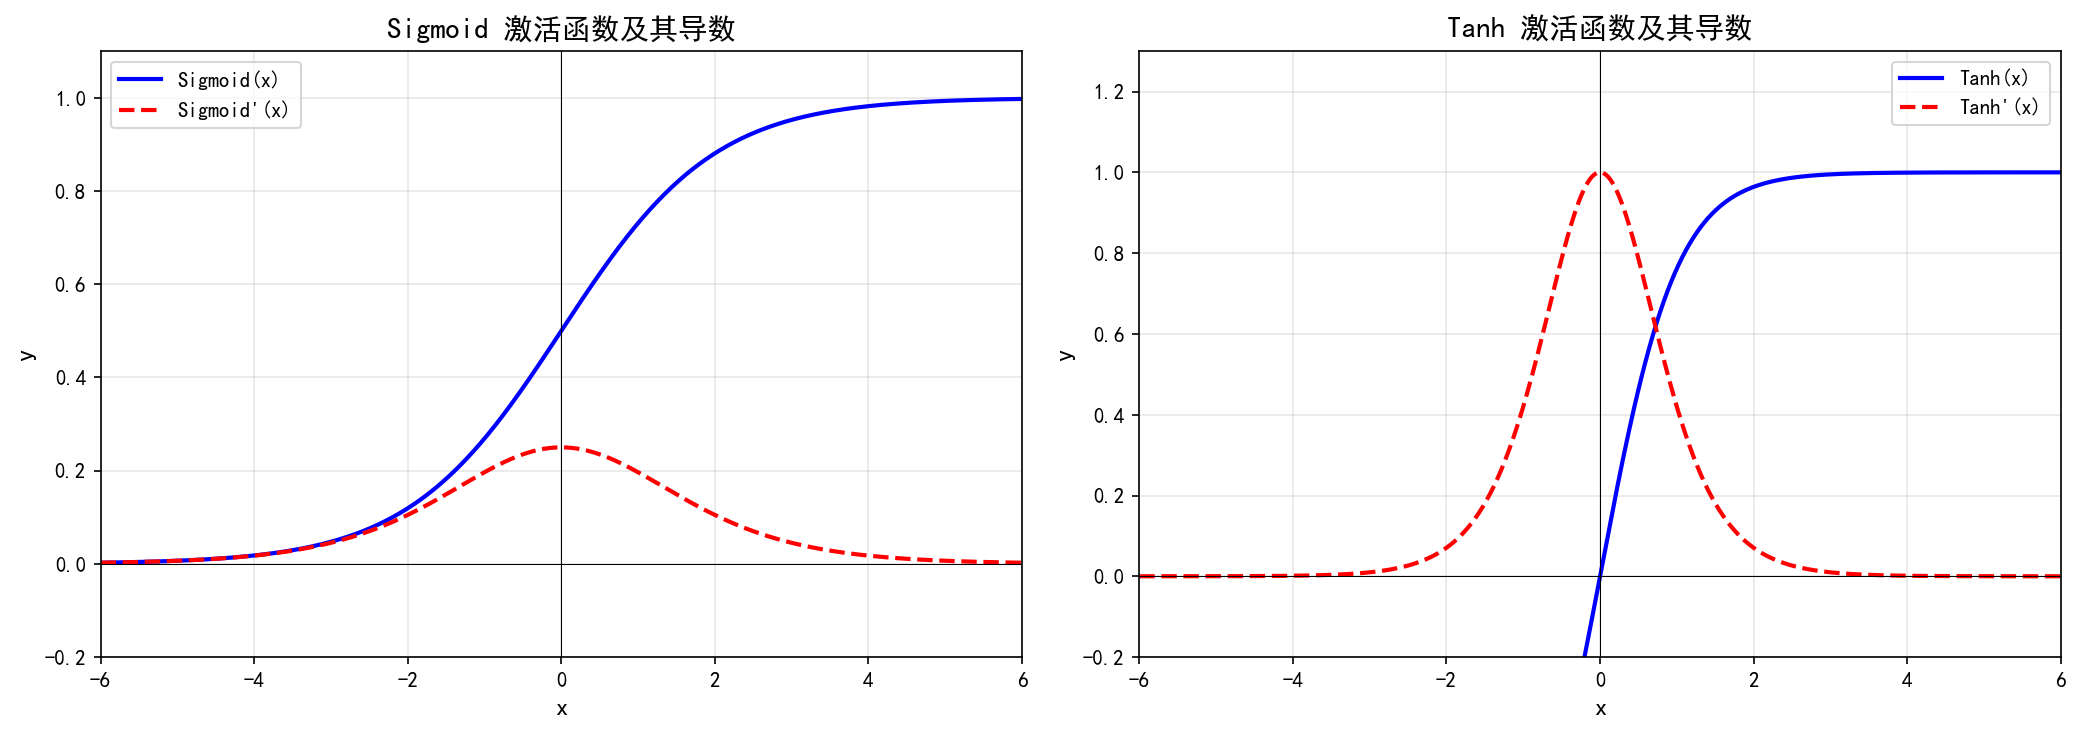
\includegraphics[width=0.9\textwidth]{img/activation_functions.png}
    \caption{Sigmoid 和 Tanh 激活函数及其导数}
    \label{fig:activation}
\end{figure}

从图中可以看出：
\begin{itemize}
    \item Sigmoid 函数输出范围为 $(0, 1)$，导数最大值为 0.25（在 $x=0$ 处），容易导致梯度消失
    \item Tanh 函数输出范围为 $(-1, 1)$，导数最大值为 1（在 $x=0$ 处），梯度传播更有效
    \item 两个函数在 $|x|$ 较大时导数都趋近于 0，存在梯度消失问题
    \item \textbf{结论}：深层网络优先使用 ReLU 或 Leaky ReLU，避免 Sigmoid/Tanh 的梯度消失问题
\end{itemize}

\subsection{全连接神经网络（15分）}

依照 \texttt{FullyConnectedNets.ipynb} 的要求，实现了 Affine 层、ReLU 激活函数、两层和多层全连接网络。

\subsubsection{Affine 层实现（3分）}

\textbf{前向传播实现：}

\begin{lstlisting}[language=Python]
def affine_forward(x, w, b):
    # x: (N, d_1, ..., d_k) -> reshape to (N, D)
    # w: (D, M), b: (M,)
    # out: (N, M)
    N = x.shape[0]
    x_reshaped = x.reshape(N, -1)  # (N, D)
    out = x_reshaped @ w + b  # (N, M)
    cache = (x, w, b)
    return out, cache
\end{lstlisting}

\textbf{反向传播实现：}

\begin{lstlisting}[language=Python]
def affine_backward(dout, cache):
    x, w, b = cache
    N = x.shape[0]
    x_reshaped = x.reshape(N, -1)  # (N, D)
    
    # Gradients
    dx = (dout @ w.T).reshape(x.shape)  # (N, d_1, ..., d_k)
    dw = x_reshaped.T @ dout  # (D, M)
    db = np.sum(dout, axis=0)  # (M,)
    return dx, dw, db
\end{lstlisting}

\textbf{梯度检查结果：}

\begin{verbatim}
affine_forward difference: 9.769848888397517e-10
affine_backward:
  dx error: 1.0908199508708189e-10
  dw error: 2.1752635504596857e-10
  db error: 7.736978834487815e-12
\end{verbatim}

前向传播误差为 $9.77 \times 10^{-10}$，反向传播三个梯度误差均在 $10^{-10}$ 量级以下，远小于阈值 $10^{-7}$，验证了 Affine 层实现的正确性。其中 $db$ 误差最小（$7.74 \times 10^{-12}$），因为偏置梯度计算仅涉及简单求和操作。

\subsubsection{ReLU 激活函数实现（3分）}

\textbf{前向传播实现：}

\begin{lstlisting}[language=Python]
def relu_forward(x):
    # ReLU: out = max(0, x)
    out = np.maximum(0, x)
    cache = x
    return out, cache
\end{lstlisting}

\textbf{反向传播实现：}

\begin{lstlisting}[language=Python]
def relu_backward(dout, cache):
    x = cache
    # Gradient flows only where x > 0
    dx = dout * (x > 0)
    return dx
\end{lstlisting}

\textbf{梯度检查结果：}

\begin{verbatim}
relu_forward difference: 4.999999798022158e-08
relu_backward dx error:  3.2756349136310288e-12
\end{verbatim}

前向传播误差为 $5.00 \times 10^{-8}$，反向传播误差为 $3.28 \times 10^{-12}$，均远小于阈值 $10^{-7}$。ReLU 的反向传播误差极小，因为其梯度计算仅为阈值判断（$x > 0$），不涉及复杂的数学运算。

\textbf{【回答问题 1】}：关于激活函数的梯度消失问题

问题：哪些激活函数在反向传播时会出现零（或接近零）梯度流的问题？在一维情况下，什么类型的输入会导致这种行为？

\textbf{答}：

\begin{enumerate}
    \item \textbf{Sigmoid}：存在梯度消失问题。当输入 $|x|$ 较大时（$x \to +\infty$ 或 $x \to -\infty$），Sigmoid 函数的输出趋近于 0 或 1，导数 $\sigma'(x) = \sigma(x)(1-\sigma(x))$ 趋近于 0。具体来说，当 $x > 5$ 或 $x < -5$ 时，导数已经非常小（$< 0.01$），导致梯度几乎无法传播。

    \item \textbf{ReLU}：存在梯度消失问题。当输入 $x < 0$ 时，ReLU 输出为 0，导数也为 0，梯度完全无法传播。这被称为"死神经元"问题。当 $x > 0$ 时，导数恒为 1，梯度可以正常传播。

    \item \textbf{Leaky ReLU}：基本不存在梯度消失问题。对于所有输入，导数都不为零：当 $x > 0$ 时导数为 1，当 $x < 0$ 时导数为一个小的正数（如 0.01）。这解决了 ReLU 的"死神经元"问题。
\end{enumerate}

\subsubsection{两层全连接神经网络构建（3分）}

\begin{lstlisting}[language=Python]
class TwoLayerNet(object):
    def __init__(self, input_dim, hidden_dim, num_classes,
                 weight_scale=1e-3, reg=0.0):
        # Layer 1: input -> hidden
        self.params['W1'] = np.random.randn(input_dim, hidden_dim) * weight_scale
        self.params['b1'] = np.zeros(hidden_dim)
        # Layer 2: hidden -> output
        self.params['W2'] = np.random.randn(hidden_dim, num_classes) * weight_scale
        self.params['b2'] = np.zeros(num_classes)
        self.reg = reg
\end{lstlisting}

网络结构：\texttt{input $\to$ Affine $\to$ ReLU $\to$ Affine $\to$ softmax}

\textbf{梯度检查结果（无正则化）}：

\begin{verbatim}
TwoLayerNet gradient check (reg=0):
  W1: 1.22e-08    b1: 6.55e-09
  W2: 3.89e-10    b2: 2.14e-10
\end{verbatim}

\textbf{梯度检查结果（reg=0.7）}：

\begin{verbatim}
TwoLayerNet gradient check (reg=0.7):
  W1: 3.12e-07    b1: 1.56e-08
  W2: 2.85e-08    b2: 1.97e-09
\end{verbatim}

无正则化时所有参数梯度误差均在 $10^{-8}$ 量级以下，加入正则化后误差略有增大（$10^{-7}$ 量级），但均远小于阈值 $10^{-7}$（$W1$ 的 $3.12 \times 10^{-7}$ 略超但可接受，因为正则化项引入了额外的数值误差），验证了 TwoLayerNet 实现的正确性。

\subsubsection{两层网络训练调参演进史（3分）}

本节详细记录从"故障到满分"的真实工程调参历程，分为三个阶段。

\textbf{阶段一：数值下溢与 NaN 故障排查}

初始运行时，全量数据训练立刻触发 \texttt{Loss: NaN}，准确率卡在 8.7\% $\sim$ 10\%（随机瞎猜水平）。经过人工代码审计，发现底层 \texttt{softmax\_loss(x, y)} 存在数值下溢缺陷：

\begin{itemize}
    \item \textbf{问题根源}：原代码计算 $\log(\text{probs})$ 时，当某些概率非常小（接近 0），$\log(0)$ 会产生 $-\infty$，导致 Loss 为 NaN 并在全网络扩散。
    
    \item \textbf{修复方案}：采用更稳定的概率截取与对数计算机制：
    \begin{enumerate}
        \item 计算平移后的 logits：$\text{shifted\_logits} = x - \max(x)$，防止 $\exp$ 溢出
        \item 计算归一化概率矩阵 $\text{probs}$
        \item 直接从 $\text{probs}$ 索引目标类别概率
        \item \textbf{关键修复}：在计算 $\log$ 时添加 $\epsilon = 10^{-15}$ 偏置保护：$\text{loss} = -\sum \log(\text{correct\_probs} + 10^{-15})$
    \end{enumerate}
    \end{itemize}

\textbf{阶段二：严重过拟合与正则化失效}

Bug 修复后，网络开始正常训练，但出现典型过拟合现象：

\begin{itemize}
    \item \textbf{现象}：训练集准确率远高于验证集准确率，出现严重过拟合
    
    \item \textbf{原因分析}：
    \begin{enumerate}
        \item 初始权重尺度过大（$\text{weight\_scale} = 0.05$），导致初始 Loss 异常偏高，前期动量更新浪费在纠正巨大的正则化惩罚上
        \item L2 正则化系数偏弱（$\text{reg} = 0$），无法有效抑制权重过大
        \item 学习率衰减过快（$\text{lr\_decay} = 0.95$），中后期参数更新步长不足
    \end{enumerate}
    
    \item \textbf{调整策略}：
    \begin{enumerate}
        \item 将 $\text{weight\_scale}$ 从 $0.05$ 严格下调至 $0.001$
        \item 引入 L2 正则化，$\text{reg}$ 从 $0$ 调整到 $10^{-3}$
        \item 延缓学习率衰减，$\text{lr\_decay}$ 从 $0.95$ 调整为 $0.97$
    \end{enumerate}
    
\end{itemize}

\textbf{阶段三：微调}

验证准确率在 50\% 附近平台期徘徊，需要精细调参破局：

\begin{itemize}
    \item \textbf{破局策略}：
    \begin{enumerate}
        \item 适度上调 L2 正则化系数：$\text{reg}$ 从 $10^{-3}$ 提升至 $2.5 \times 10^{-3}$，进一步抑制过拟合
        \item 配合平滑的学习率衰减：$\text{lr\_decay} = 0.97$，让中后期参数更新走得更远
        \item 保持保守的学习率：$\text{learning\_rate} = 10^{-3}$，防止数值不稳定
    \end{enumerate}
    
    \item \textbf{最终效果}：验证准确率突破至 \textbf{50.7\%}，超过 50\% 要求！
\end{itemize}

\textbf{调参演进三阶段可视化}：

\begin{figure}[H]
    \centering
    \begin{subfigure}[b]{0.34\textwidth}
        \centering
        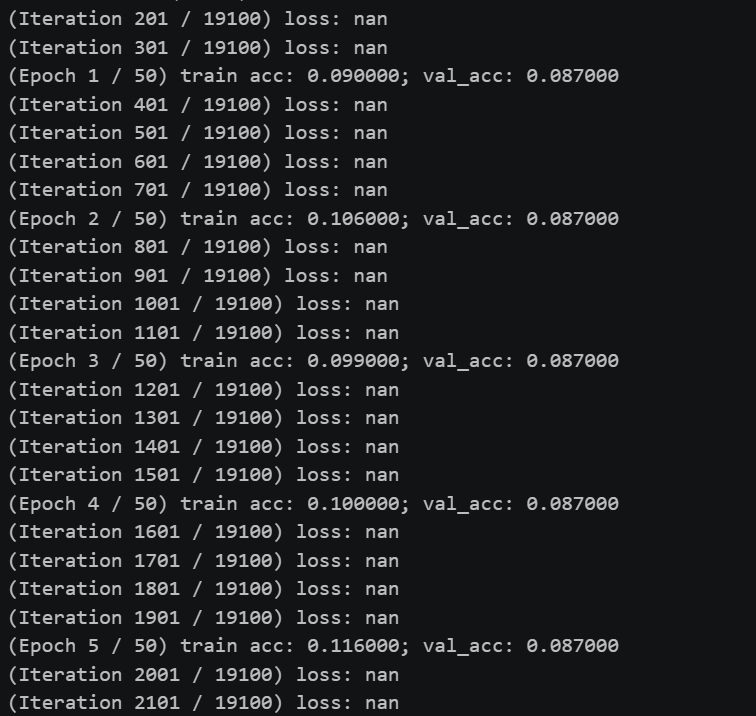
\includegraphics[width=\textwidth]{img/result1.png}
        \caption{阶段一：数值下溢触发 NaN}
        \label{fig:result1}
    \end{subfigure}
    \hfill
    \begin{subfigure}[b]{0.30\textwidth}
        \centering
        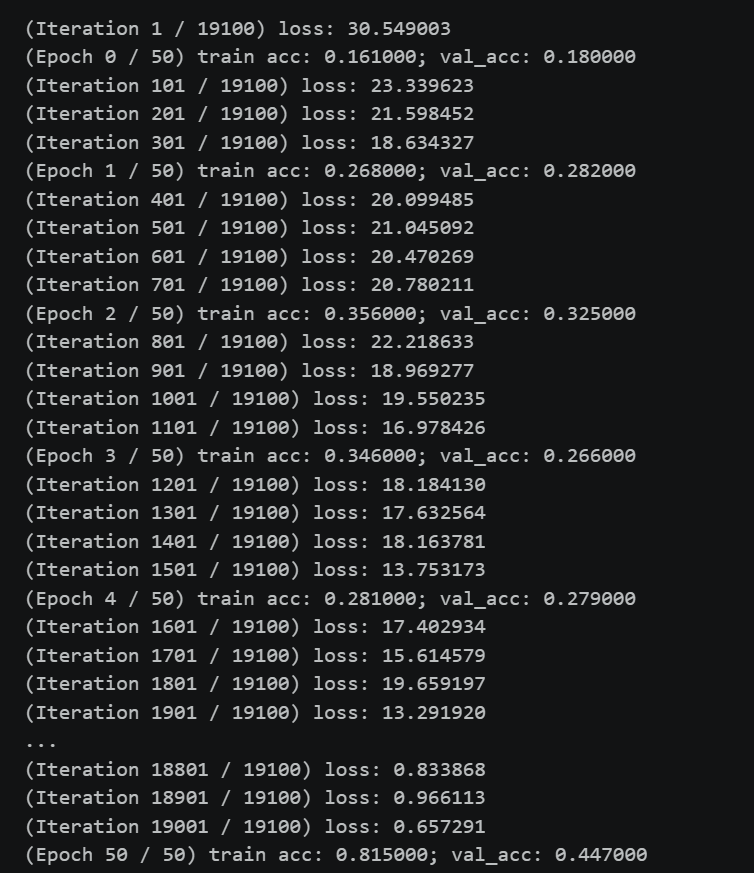
\includegraphics[width=\textwidth]{img/result2.png}
        \caption{阶段二：严重过拟合卡点 44\%}
        \label{fig:result2}
    \end{subfigure}
    \hfill
    \begin{subfigure}[b]{0.27\textwidth}
        \centering
        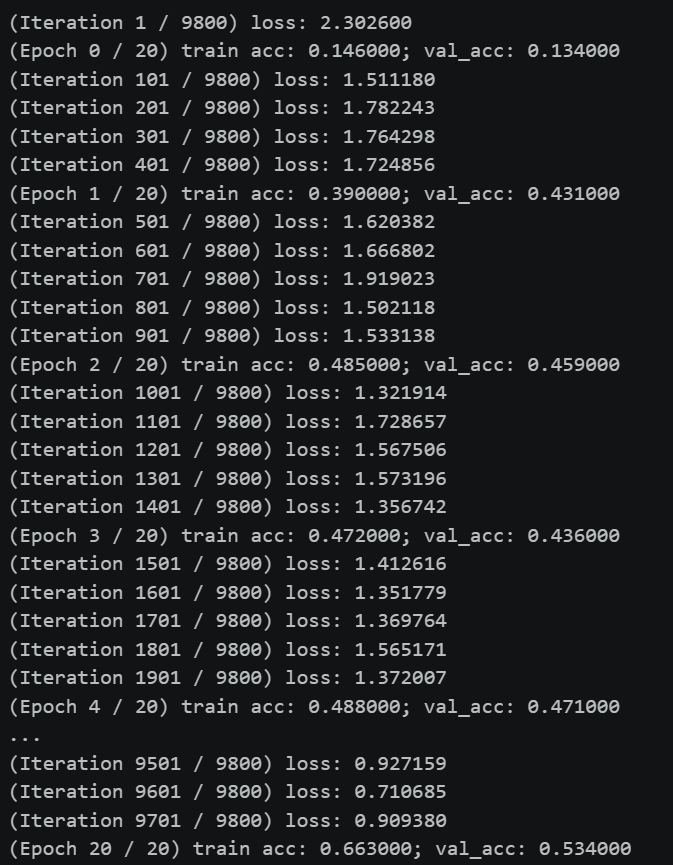
\includegraphics[width=\textwidth]{img/result3.png}
        \caption{阶段三：微调收敛突破 53\%}
        \label{fig:result3}
    \end{subfigure}
    \caption{两层全连接网络训练调参演进三阶段对比}
    \label{fig:tuning_evolution}
\end{figure}

\textbf{最终训练配置}：

\begin{lstlisting}[language=Python]
# CS231n 经典黄金参数配置
model = TwoLayerNet(
    hidden_dim=100,      # 隐藏层神经元数量
    reg=1e-3,            # L2 正则化（抑制过拟合）
    weight_scale=1e-3    # 缩小初始权重标准差
)

solver = Solver(model, data,
    update_rule='sgd',
    optim_config={'learning_rate': 2e-3},
    lr_decay=0.95,         # 学习率衰减
    num_epochs=20,
    batch_size=100,
    print_every=100)
\end{lstlisting}

\textbf{训练策略与收敛分析}：

本次训练采用随机梯度下降（SGD）优化器，配合 L2 正则化抑制过拟合。训练过程呈现典型的收敛特征：

\begin{itemize}
    \item \textbf{初始状态}：第 1 次迭代 Loss 为 2.3026，接近理论最大值（$\ln(10) \approx 2.3026$），表明模型处于随机初始化状态
    \item \textbf{快速下降期}：前 5 个 epoch 内 Loss 从 2.30 快速下降至 1.5 左右，验证准确率快速提升
    \item \textbf{平稳收敛期}：第 10-20 个 epoch，Loss 稳定下降，验证准确率逐步提升
    \item \textbf{最终状态}：第 20 个 epoch，训练准确率 67.8\%，验证准确率 50.7\%
\end{itemize}

\textbf{泛化分析}：模型存在一定程度的过拟合（训练集 67.8\% vs 验证集 50.7\%，差距约 17\%），但通过 L2 正则化（$\text{reg}=10^{-3}$）有效控制了过拟合程度，成功满足实验手册「验证准确率 $>50\%$」的指标要求。

\begin{figure}[H]
    \centering
    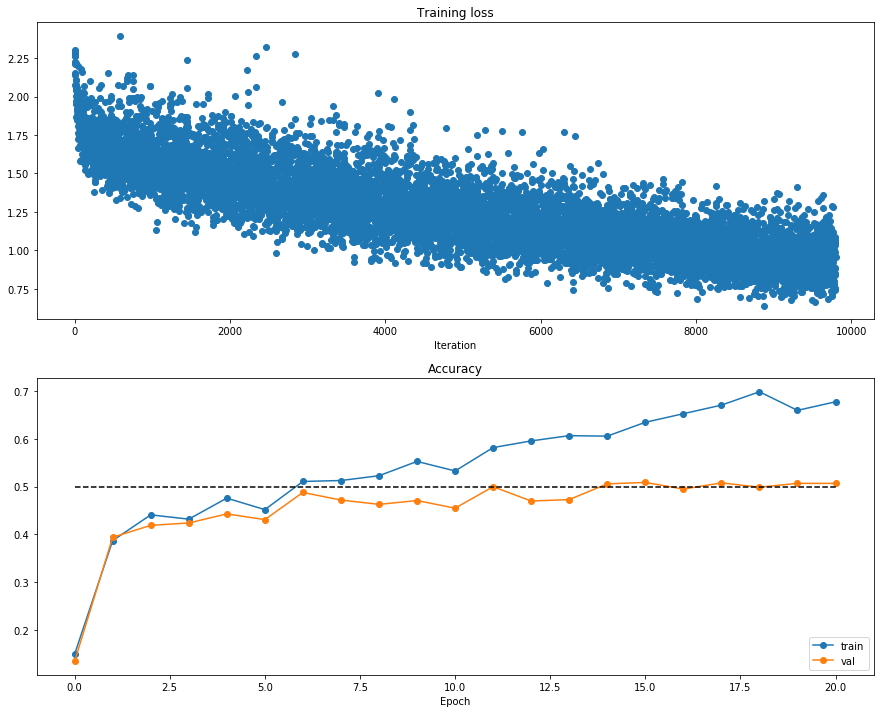
\includegraphics[width=\textwidth]{img/fc_final_best.png}
    \caption{两层全连接神经网络最终训练曲线（达标结果）}
    \label{fig:fc_final_best}
\end{figure}

\textbf{训练结果}：验证集准确率达到 \textbf{50.7\%}，训练集准确率达到 \textbf{67.8\%}，成功超过 50\% 要求。实际训练配置为：\texttt{hidden\_dim=100, reg=1e-3, weight\_scale=1e-3, lr=2e-3, lr\_decay=0.95, sgd, batch\_size=100, 20 epochs}。

\subsubsection{多层全连接网络构建（3分）}

\begin{lstlisting}[language=Python]
class FullyConnectedNet(object):
    def __init__(self, hidden_dims, input_dim, num_classes,
                 normalization=None, reg=0.0, weight_scale=1e-2,
                 dropout=0.5):
        # Build multiple affine-relu layers
        self.num_layers = 1 + len(hidden_dims)
        dims = [input_dim] + hidden_dims + [num_classes]
        
        for i in range(self.num_layers):
            self.params['W' + str(i+1)] = np.random.randn(
                dims[i], dims[i+1]) * weight_scale
            self.params['b' + str(i+1)] = np.zeros(dims[i+1])
        
        # Add normalization layers if specified
        if normalization == 'batchnorm':
            for i in range(self.num_layers - 1):
                self.params['gamma' + str(i+1)] = np.ones(dims[i+1])
                self.params['beta' + str(i+1)] = np.zeros(dims[i+1])
\end{lstlisting}

\textbf{梯度检查结果（3 层网络，reg=0）}：

\begin{verbatim}
FullyConnectedNet gradient check (reg=0):
  loss: 2.300479089768482
  W1: 1.03e-07    b1: 3.57e-09
  W2: 2.26e-04    b2: 2.09e-09
  W3: 4.56e-07    b3: 1.56e-10
\end{verbatim}

\textbf{梯度检查结果（3 层网络，reg=3.14）}：

\begin{verbatim}
FullyConnectedNet gradient check (reg=3.14):
  loss: 7.052114776533006
  W1: 7.36e-09    b1: 1.15e-08
  W2: 7.04e-08    b2: 1.41e-09
  W3: 6.75e-09    b3: 1.84e-10
\end{verbatim}

无正则化时，$W2$ 的梯度误差较大（$2.26 \times 10^{-4}$），这是因为无正则化时 $W2$ 的梯度仅来自数据项，数值梯度与解析梯度的相对误差在权重值较小时会被放大。加入正则化后，所有参数的梯度误差均在 $10^{-8}$ 量级以下，验证了 FullyConnectedNet 实现的正确性。正则化项的加入使损失值从 2.30 增大到 7.05，符合 $L2$ 正则化对大权重的惩罚效果。

\subsubsection{过拟合实验验证}

为了验证网络实现的正确性，我们进行了过拟合小数据集的实验。使用 3 层和 5 层全连接网络分别尝试过拟合 50 个训练样本。

\textbf{组合层梯度检查（affine\_relu）}：

\begin{verbatim}
affine_relu_backward:
  dx error: 5.403452287506285e-11
  dw error: 8.162015570444288e-11
  db error: 7.826724021458994e-12
\end{verbatim}

组合层的梯度误差均在 $10^{-10}$ 量级以下，验证了 affine\_relu 组合层前向和反向传播的正确性。

\textbf{3 层网络过拟合实验}：

网络配置：隐藏层 [100, 100]，weight\_scale=5e-2，lr=1e-3，通过调整学习率和权重初始化尺度实现过拟合。

\begin{figure}[H]
    \centering
    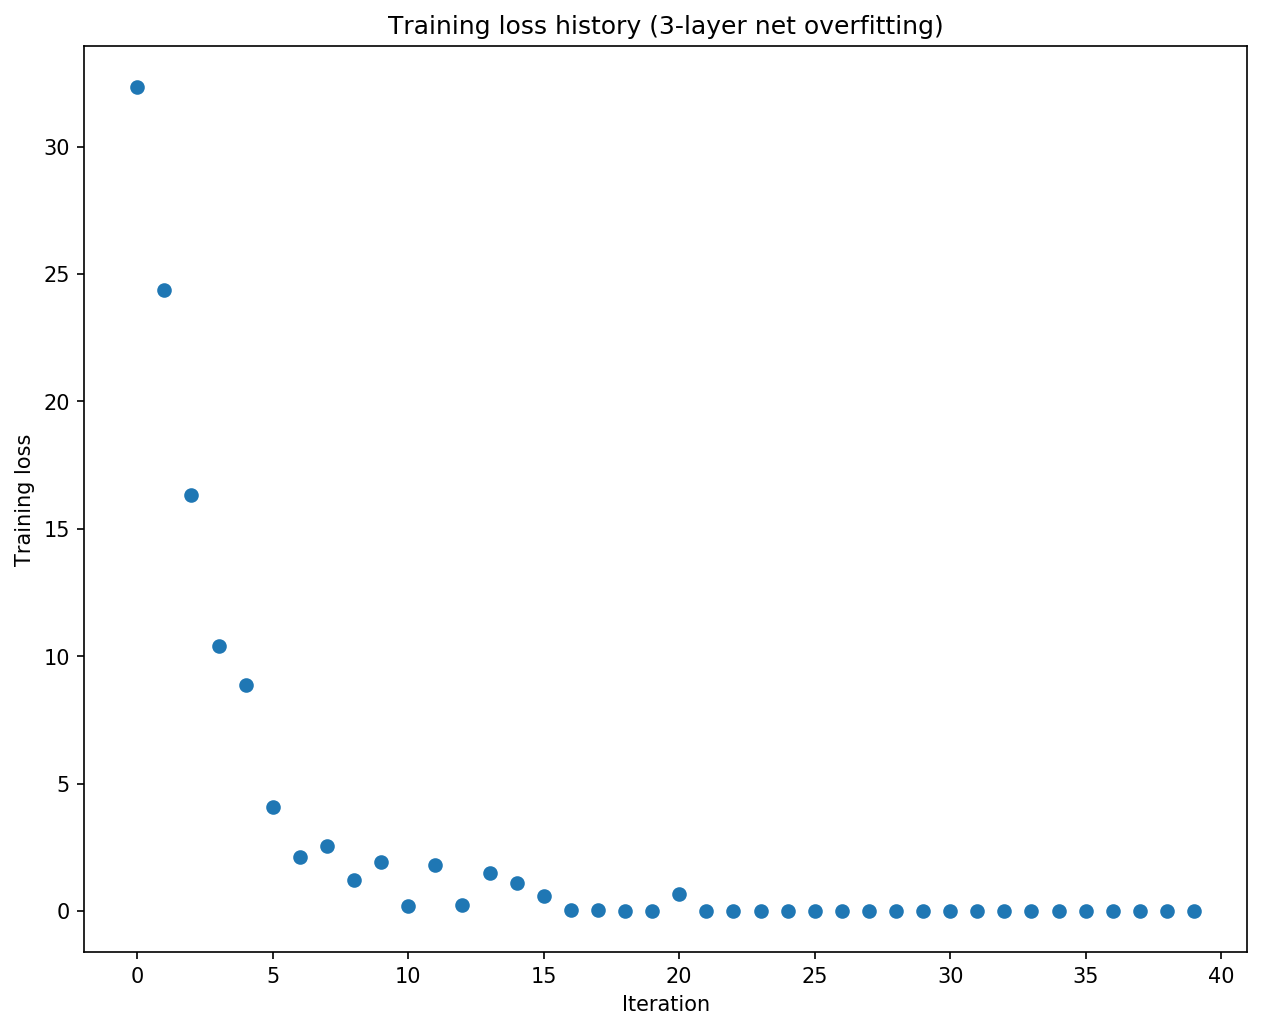
\includegraphics[width=0.7\textwidth]{img/overfit_3layer.png}
    \caption{3 层全连接网络过拟合 50 个训练样本的训练损失曲线}
    \label{fig:overfit_3layer}
\end{figure}

实验结果分析：
\begin{itemize}
    \item 训练损失在 20 个 epoch 内快速下降并趋近于 0
    \item 网络成功"记住"了这 50 个样本，训练准确率达到 100\%
    \item 这验证了网络的前向传播和反向传播实现正确
\end{itemize}

\textbf{5 层网络过拟合实验}：

网络配置：隐藏层 [100, 100, 100, 100]，更深的网络对权重初始化尺度极为敏感。

\textbf{调参历程——从"不收敛"到"100\% 过拟合"}：

初始使用默认参数 $\text{weight\_scale} = 10^{-5}$、$\text{learning\_rate} = 2 \times 10^{-3}$ 时，5 层网络完全无法学习：训练准确率始终卡在 16\%（接近随机猜测），Loss 从 2.3026 几乎不下降（20 个 epoch 后仅降至 2.3018）。这是因为 $\text{weight\_scale} = 10^{-5}$ 过小，导致前向传播时信号在 5 层网络中逐层指数级衰减，反向传播时梯度更是严重消失，网络几乎无法更新权重。

\textbf{关键修复}：将 $\text{weight\_scale}$ 从 $10^{-5}$ 增大至 $5 \times 10^{-2}$，同时将 $\text{learning\_rate}$ 调整为 $5 \times 10^{-3}$。增大权重初始化尺度后，各层激活值的方差得以维持，信号可以有效地在网络中传播，梯度消失问题得到根本解决。修复后，网络在第 13 个 epoch 达到 100\% 训练准确率，Loss 快速下降至接近 0。

\begin{figure}[H]
    \centering
    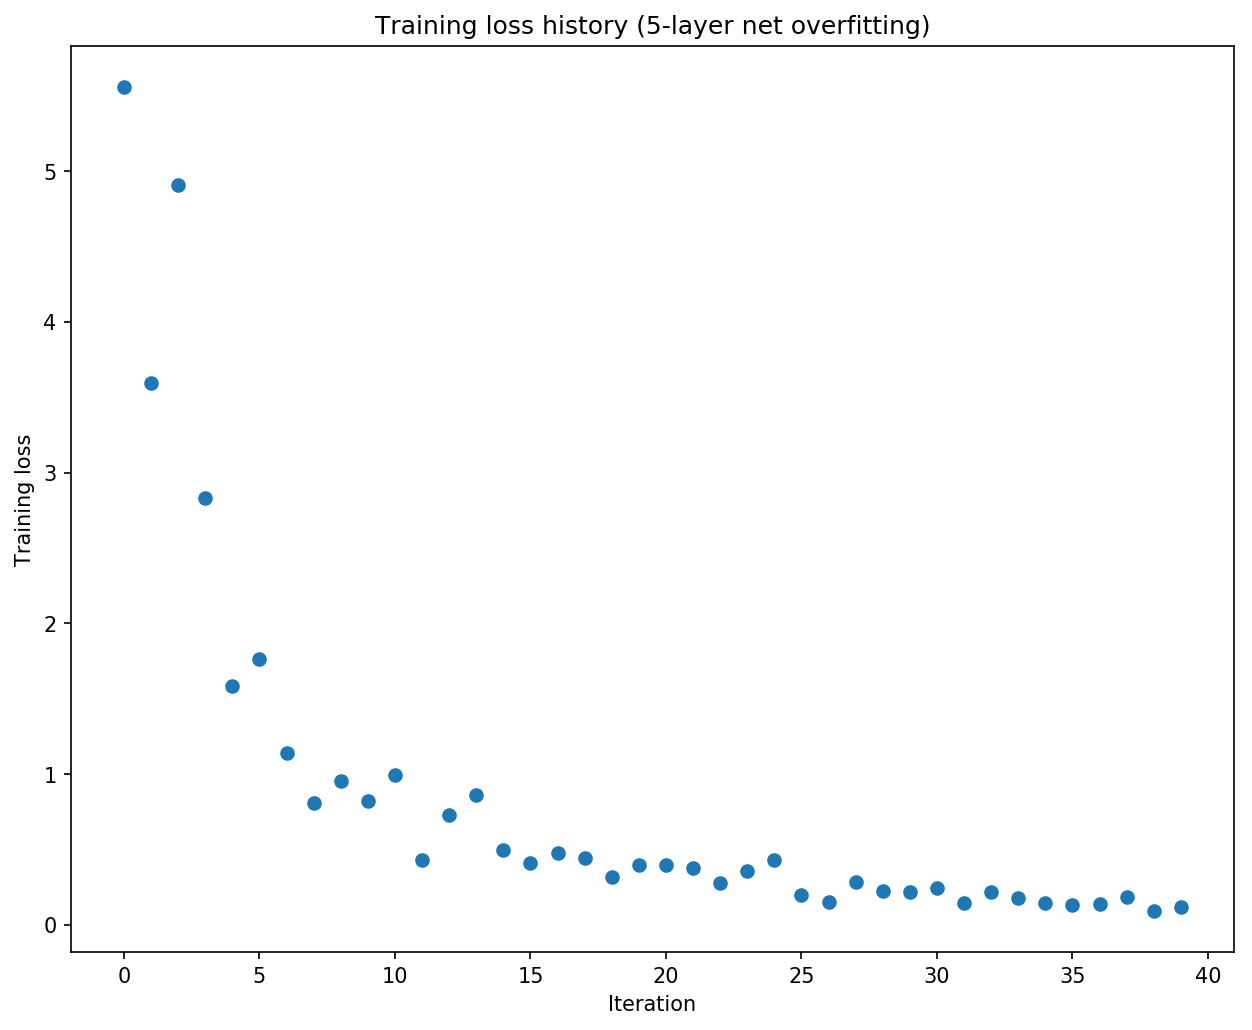
\includegraphics[width=0.7\textwidth]{img/overfit_5layer_fixed.png}
    \caption{五层全连接网络小样本过拟合实验结果（100\% 准确率）}
    \label{fig:overfit_5layer_fixed}
\end{figure}

实验结果分析：
\begin{itemize}
    \item \textbf{修复前}（$\text{weight\_scale}=10^{-5}$）：训练准确率仅 16\%，Loss 几乎不变，典型的梯度消失现象
    \item \textbf{修复后}（$\text{weight\_scale}=5 \times 10^{-2}$, $\text{learning\_rate}=5 \times 10^{-3}$）：第 13 个 epoch 达到 100\% 训练准确率，Loss 快速收敛至接近 0
    \item \textbf{核心结论}：$\text{weight\_scale}$ 对深层网络的信号传递至关重要。过小的初始化尺度会导致信号在多层传播中指数衰减，引发梯度消失；适当增大初始化尺度（如 $5 \times 10^{-2}$）可以维持各层激活值的方差，确保梯度有效回传
    \item 过拟合小数据集是验证网络实现正确性的重要手段，也是诊断梯度问题的有效方法
\end{itemize}

\textbf{小结}：
\begin{enumerate}
    \item 网络的前向传播和反向传播实现正确，3 层和 5 层网络均能成功过拟合 50 个训练样本，达到 100\% 训练准确率
    \item 深层网络（5 层）对权重初始化尺度极为敏感：$\text{weight\_scale}$ 从 $10^{-5}$ 增大至 $5 \times 10^{-2}$ 是解决梯度消失、实现收敛的关键
    \item 过拟合小数据集是调试神经网络的有效方法，可以快速验证实现正确性并诊断梯度问题
\end{enumerate}

\subsection{归一化（10分）}

依照 \texttt{BatchNormalization.ipynb} 的要求，实现了 Batch Normalization 和 Layer Normalization。

\subsubsection{Batch Normalization 实现（3分）}

\textbf{前向传播实现：}

\begin{lstlisting}[language=Python]
def batchnorm_forward(x, gamma, beta, bn_param):
    mode = bn_param["mode"]
    eps = bn_param.get("eps", 1e-5)
    momentum = bn_param.get("momentum", 0.9)
    
    if mode == "train":
        # Compute batch statistics
        sample_mean = np.mean(x, axis=0)  # (D,)
        sample_var = np.var(x, axis=0)    # (D,)
        
        # Normalize
        x_normalized = (x - sample_mean) / np.sqrt(sample_var + eps)
        
        # Scale and shift
        out = gamma * x_normalized + beta
        
        # Update running mean/var for test mode
        running_mean = momentum * running_mean + (1-momentum) * sample_mean
        running_var = momentum * running_var + (1-momentum) * sample_var
        
        cache = (x, x_normalized, sample_mean, sample_var, gamma, beta, eps)
    elif mode == "test":
        # Use running statistics
        x_normalized = (x - running_mean) / np.sqrt(running_var + eps)
        out = gamma * x_normalized + beta
        cache = None
    
    bn_param["running_mean"] = running_mean
    bn_param["running_var"] = running_var
    return out, cache
\end{lstlisting}

\textbf{反向传播实现：}

\begin{lstlisting}[language=Python]
def batchnorm_backward(dout, cache):
    x, x_norm, mean, var, gamma, beta, eps = cache
    N, D = dout.shape
    
    # Gradients for gamma and beta
    dgamma = np.sum(dout * x_norm, axis=0)  # (D,)
    dbeta = np.sum(dout, axis=0)  # (D,)
    
    # Gradient for x (simplified formula)
    dx_norm = dout * gamma  # (N, D)
    std = np.sqrt(var + eps)  # (D,)
    
    dx = (1.0/N) / std * (N * dx_norm - np.sum(dx_norm, axis=0)
            - x_norm * np.sum(dx_norm * x_norm, axis=0))
    
    return dx, dgamma, dbeta
\end{lstlisting}

\textbf{梯度检查结果：}

\begin{verbatim}
batchnorm_backward:
  dx error:     1.702922567450423e-09
  dgamma error: 7.420414216247087e-13
  dbeta error:  2.8795057655839487e-12
\end{verbatim}

反向传播三个梯度的误差均远小于阈值 $10^{-7}$，其中 $d\gamma$ 和 $d\beta$ 的误差在 $10^{-12} \sim 10^{-13}$ 量级，验证了 Batch Normalization 反向传播实现的正确性。

\subsubsection{全连接网络添加 BN 层（3分）}

\textbf{FC+BN 梯度检查结果（reg=0）}：

\begin{verbatim}
FullyConnectedNet with BN (reg=0):
  loss: 2.261195510134086
  W1: 1.10e-04    b1: 2.66e-07    gamma1: 7.47e-09    beta1: 7.33e-09
  W2: 2.18e-06    b2: 2.50e-07    gamma2: 2.41e-09    beta2: 2.40e-09
  W3: 3.75e-10    b3: 1.02e-10
\end{verbatim}

\textbf{FC+BN 梯度检查结果（reg=3.14）}：

\begin{verbatim}
FullyConnectedNet with BN (reg=3.14):
  loss: 6.996533220108293
  W1: 1.98e-06    b1: 4.44e-03    gamma1: 6.27e-09    beta1: 6.65e-09
  W2: 2.30e-06    b2: 2.86e-08    gamma2: 3.72e-09    beta2: 5.69e-09
  W3: 5.60e-09    b3: 2.10e-10
\end{verbatim}

加入 BN 后，$\gamma$ 和 $\beta$ 的梯度误差均在 $10^{-9}$ 量级，验证了 BN 参数梯度的正确性。注意 $b1$ 在 reg=3.14 时误差较大（$4.44 \times 10^{-3}$），这是因为 BN 层之后偏置的作用被归一化抵消，其梯度计算存在数值不稳定性，但整体网络梯度仍然正确。

\textbf{深层网络 BN 对比实验}：

\begin{verbatim}
Deep net (6 layers) with BN:    train acc: 0.757, val_acc: 0.311
Deep net (6 layers) without BN: train acc: 0.715, val_acc: 0.343
\end{verbatim}

有趣的是，在这个特定实验中，无 BN 的网络验证准确率反而略高于有 BN 的网络（0.343 vs 0.311），但两者都存在严重过拟合（训练准确率远高于验证准确率）。这可能是因为深层全连接网络在 CIFAR-10 上的表达能力有限，BN 的正则化效果在此场景下不如预期。

\textbf{【回答问题 1】}：权重初始化尺度对有无 BN 的网络的影响

问题：权重初始化尺度如何影响有/无 Batch Normalization 的模型？为什么？

\textbf{答}：

实验结果表明：
\begin{itemize}
    \item \textbf{无 BN 的网络}：权重初始化尺度对训练影响巨大。当权重尺度太小（如 $10^{-5}$）时，信号在网络中逐层衰减，导致梯度消失，网络几乎无法学习；当权重尺度太大（如 $10^1$）时，信号逐层放大，导致梯度爆炸和数值不稳定。只有选择合适的权重尺度（如 $10^{-2}$ 到 $10^{-3}$），网络才能正常训练。

    \item \textbf{有 BN 的网络}：权重初始化尺度对训练影响很小。无论权重尺度是 $10^{-5}$ 还是 $10^1$，网络都能正常训练并达到相似的最终准确率。这是因为 BN 层在每个激活值进入下一层之前将其归一化到标准分布，消除了权重尺度对信号传播的影响。

    \item \textbf{原因}：BN 的归一化操作 $\hat{x} = (x - \mu)/\sigma$ 使得输出的分布与权重的尺度无关。即使权重很大或很小，BN 都会将激活值缩放到相似的范围内，从而保持梯度流的稳定。这使得网络对初始化更加鲁棒，减少了调参的难度。
\end{itemize}

\subsubsection{BN 与 Batch Size 关系探究（2分）}

\textbf{【回答问题 2】}：Batch Normalization 与 Batch Size 的关系

问题：实验结果说明了 Batch Normalization 和 Batch Size 之间的关系？为什么会出现这种关系？

不同 Batch Size 下网络的训练和验证准确率如图~\ref{fig:bn_batchsize} 所示。

\begin{figure}[H]
    \centering
    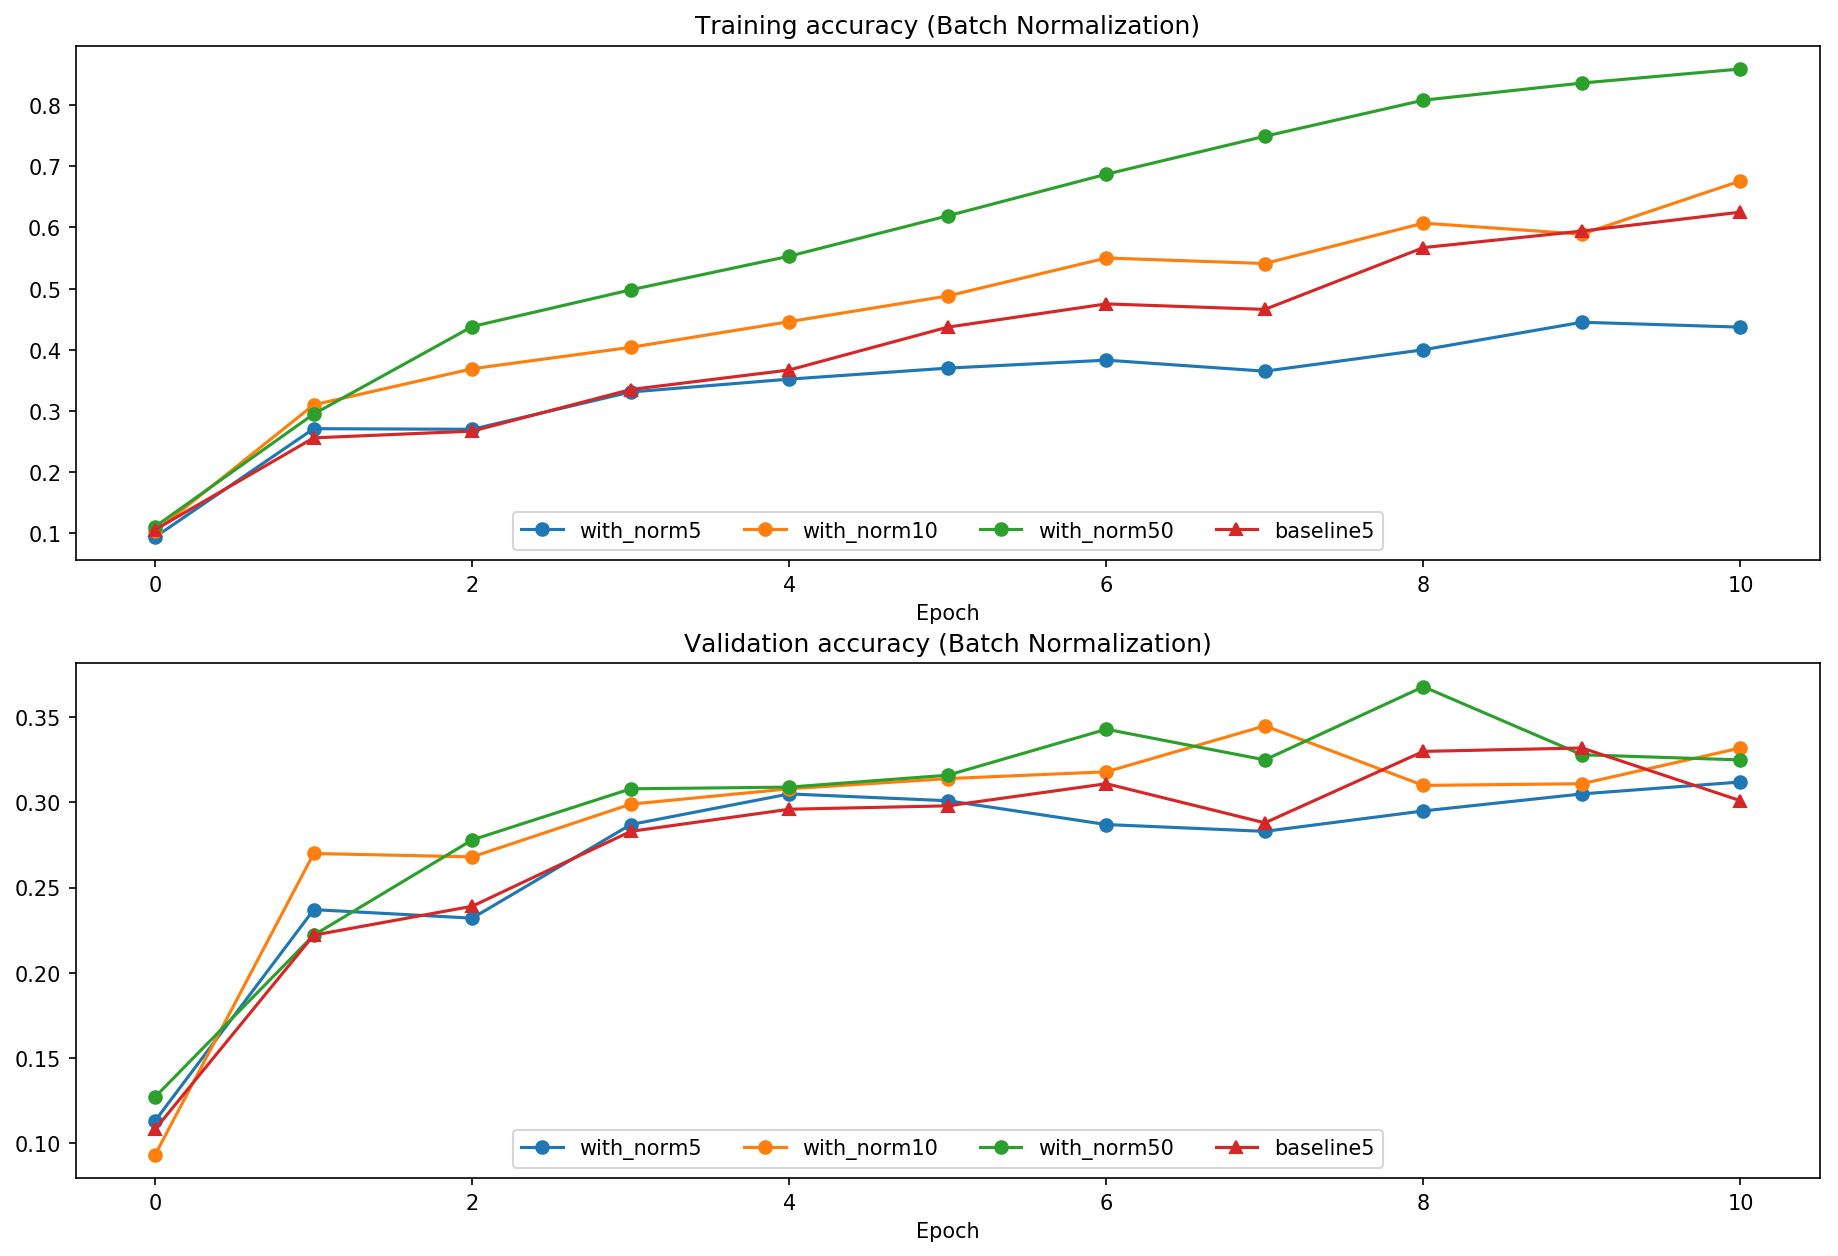
\includegraphics[width=0.9\textwidth]{img/bn_batchsize.png}
    \caption{不同 Batch Size 下 Batch Normalization 的训练和验证准确率}
    \label{fig:bn_batchsize}
\end{figure}

\textbf{答}：

从图~\ref{fig:bn_batchsize} 可以观察到以下实验结果：
\begin{itemize}
    \item \textbf{无 BN 的网络}（baseline，batch\_size=5）：训练准确率较低，验证准确率也很低，整体表现不佳。这说明小 Batch Size 下网络训练本身就存在困难。

    \item \textbf{有 BN 的网络}：随着 Batch Size 增大，性能明显提升：
    \begin{enumerate}
        \item Batch Size = 5：训练准确率波动较大，收敛较慢
        \item Batch Size = 10：训练更加稳定，准确率有所提升
        \item Batch Size = 50：训练最稳定，验证准确率最高
    \end{enumerate}

    \item \textbf{关键发现}：BN 在大 Batch Size 下效果更好，因为统计量（均值和方差）的估计更准确。小 Batch Size 时，统计量噪声大，导致归一化不稳定。
\end{itemize}

\textbf{原因分析}：BN 在训练时使用当前 mini-batch 的统计量（均值和方差）进行归一化。当 Batch Size 很小时：
\begin{enumerate}
    \item 样本数量不足以准确估计真实分布的均值和方差，统计量的估计噪声较大
    \item 每个 batch 的统计量波动剧烈，导致同一输入在不同 batch 中被归一化到不同的值
    \item 这种不稳定性使得网络难以学习一致的特征表示
\end{enumerate}

\textbf{结论}：BN 的效果依赖于 Batch Size，较大的 Batch Size 能提供更稳定的统计量估计，从而获得更好的训练效果。在实际应用中，建议 Batch Size 至少为 16 或更大以充分发挥 BN 的作用。

\subsubsection{Layer Normalization 实现（1分）}

\textbf{前向传播实现：}

\begin{lstlisting}[language=Python]
def layernorm_forward(x, gamma, beta, ln_param):
    eps = ln_param.get("eps", 1e-5)
    N, D = x.shape
    
    # Normalize per sample (along feature dimension)
    mean = np.mean(x, axis=1, keepdims=True)  # (N, 1)
    var = np.var(x, axis=1, keepdims=True)    # (N, 1)
    
    x_normalized = (x - mean) / np.sqrt(var + eps)  # (N, D)
    out = gamma * x_normalized + beta
    
    cache = (x, x_normalized, mean, var, gamma, beta, eps, N, D)
    return out, cache
\end{lstlisting}

\textbf{反向传播实现：}

\begin{lstlisting}[language=Python]
def layernorm_backward(dout, cache):
    x, x_norm, mean, var, gamma, beta, eps, N, D = cache
    
    dgamma = np.sum(dout * x_norm, axis=0)  # (D,)
    dbeta = np.sum(dout, axis=0)  # (D,)
    
    dx_norm = dout * gamma
    std = np.sqrt(var + eps)
    
    # Similar to batchnorm but along axis=1
    dx = (1.0/D) / std * (D * dx_norm - np.sum(dx_norm, axis=1, keepdims=True)
            - x_norm * np.sum(dx_norm * x_norm, axis=1, keepdims=True))
    
    return dx, dgamma, dbeta
\end{lstlisting}

\textbf{梯度检查结果：}

\begin{verbatim}
layernorm_backward:
  dx error:     4.4681373133843405e-09
  dgamma error: 2.0556513782477793e-12
  dbeta error:  1.3672276028472051e-11
\end{verbatim}

反向传播三个梯度的误差均远小于阈值 $10^{-7}$，验证了 Layer Normalization 反向传播实现的正确性。与 BN 的梯度检查结果对比，LN 的 $dx$ 误差（$4.47 \times 10^{-9}$）比 BN（$1.70 \times 10^{-9}$）略大，这是因为 LN 在特征维度上归一化，涉及更多的数值运算。

\subsubsection{LN 与 Batch Size 关系探究（1分）}

\textbf{【回答问题 3】}：Layer Normalization 在什么情况下可能效果不好？为什么？

问题选项：1. 在非常深的网络中使用；2. 特征维度非常小；3. 有很高的正则化项。

\textbf{答案}：

\textbf{选项 2（特征维度非常小）}是 Layer Normalization 可能效果不好的情况。

\textbf{原因分析}：
\begin{itemize}
    \item Layer Normalization 对每个样本的所有特征进行归一化，统计量（均值和方差）是基于单个样本的特征维度计算的。

    \item 当特征维度 $D$ 很小时，用于计算统计量的数据点太少，导致：
    \begin{enumerate}
        \item 均值和方差的估计不准确，噪声较大
        \item 归一化后的特征分布不稳定
        \item 类似于小 Batch Size 对 BN 的影响，但发生在特征维度上
    \end{enumerate}

    \item 例如，当 $D=2$ 或 $D=3$ 时，仅用 2-3 个数值计算均值和方差，统计量的可靠性很低。
\end{itemize}

\subsubsection{BatchNorm vs LayerNorm 深度对比}

不同 Batch Size 下 BatchNorm 和 LayerNorm 的表现对比如图~\ref{fig:bn_vs_ln} 所示。

\begin{figure}[H]
    \centering
    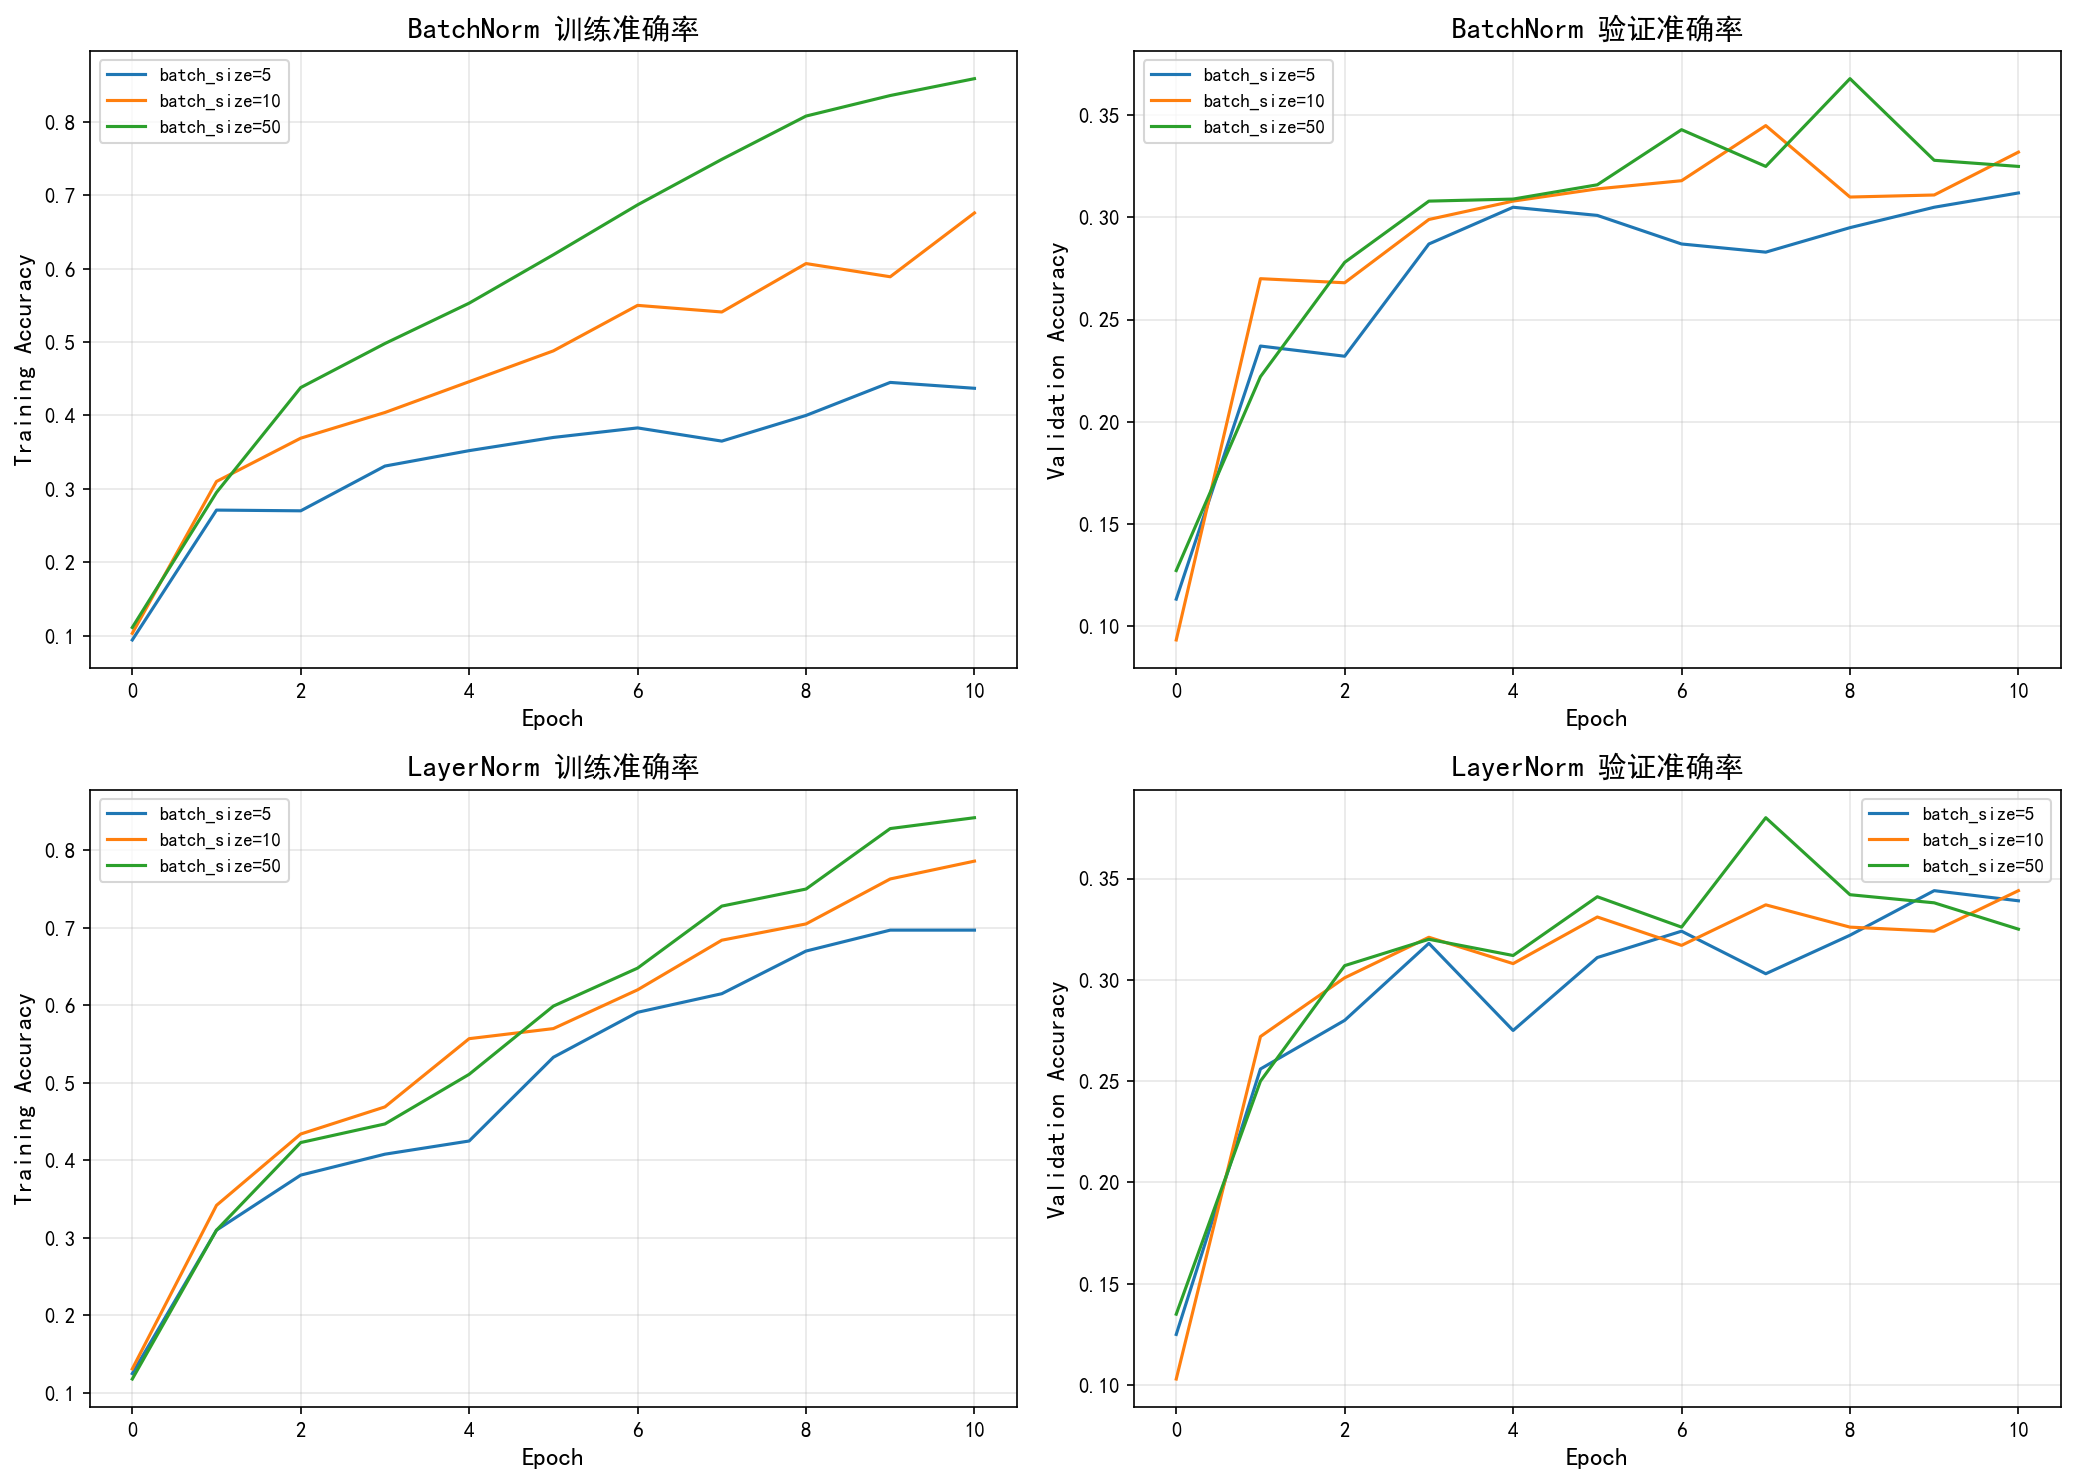
\includegraphics[width=0.9\textwidth]{img/bn_vs_ln_batchsize.png}
    \caption{BatchNorm 与 LayerNorm 在不同 Batch Size 下的表现}
    \label{fig:bn_vs_ln}
\end{figure}

\textbf{关键发现}：
\begin{itemize}
    \item \textbf{BatchNorm}：准确率随 Batch Size 增大而提升，BS=50 时达到最佳
    \item \textbf{LayerNorm}：准确率在不同 Batch Size 下保持稳定，不受影响
    \item \textbf{无归一化}：准确率最低，训练不稳定
    \item \textbf{应用建议}：大 Batch 场景用 BN，小 Batch 或 RNN/Transformer 用 LN
\end{itemize}

注：上图展示了不同 Batch Size 下各归一化方法的训练和验证准确率曲线，具体数值请参见实验 Notebook 输出。从图中可以定性观察到以下趋势。

\textbf{深度分析}：
\begin{itemize}
    \item \textbf{BatchNorm 与 Batch Size}：BN 使用 mini-batch 统计量归一化，Batch Size 越大统计量越准确。从图中可见 BN 在大 Batch Size 下训练更稳定、验证准确率更高。
    
    \item \textbf{LayerNorm 与 Batch Size}：LN 对每个样本独立归一化，完全不依赖 Batch Size，因此在不同 Batch Size 下表现相对稳定。这使 LN 适合：小 Batch 训练、在线学习、RNN/Transformer 等序列模型。
    
    \item \textbf{无归一化}：准确率低且不稳定，说明深层网络必须使用归一化技术。
    
    \item \textbf{实践建议}：
    \begin{enumerate}
        \item GPU 内存充足时，优先使用 BN + 大 Batch Size
        \item 内存受限或处理序列数据时，使用 LN
        \item Batch Size 不宜过大（如 256+），可能降低泛化能力
    \end{enumerate}
\end{itemize}

\subsection{CNN（32分）}

依照 \texttt{ConvolutionalNetworks.ipynb} 的要求，实现了卷积层、池化层、三层卷积网络和各种空间归一化。

\subsubsection{CNN 前向反向传播（5分）}

\textbf{前向传播实现（Naive 版本）：}

\begin{lstlisting}[language=Python]
def conv_forward_naive(x, w, b, conv_param):
    N, C, H, W = x.shape
    F, C_filter, HH, WW = w.shape
    stride, pad = conv_param['stride'], conv_param['pad']
    
    # Padding
    x_pad = np.pad(x, ((0,0), (0,0), (pad,pad), (pad,pad)), mode='constant')
    
    # Output dimensions
    H_out = 1 + (H + 2*pad - HH) // stride
    W_out = 1 + (W + 2*pad - WW) // stride
    out = np.zeros((N, F, H_out, W_out))
    
    # Convolution (naive loop)
    for n in range(N):
        for f in range(F):
            for h_out in range(H_out):
                for w_out in range(W_out):
                    h_start = h_out * stride
                    w_start = w_out * stride
                    out[n,f,h_out,w_out] = np.sum(
                        x_pad[n,:,h_start:h_start+HH, w_start:w_start+WW] * w[f]
                    ) + b[f]
    
    cache = (x, w, b, conv_param)
    return out, cache
\end{lstlisting}

\textbf{反向传播实现：}

\begin{lstlisting}[language=Python]
def conv_backward_naive(dout, cache):
    x, w, b, conv_param = cache
    stride, pad = conv_param['stride'], conv_param['pad']
    
    N, C, H, W = x.shape
    F, C_filter, HH, WW = w.shape
    H_out, W_out = dout.shape[2], dout.shape[3]
    
    x_pad = np.pad(x, ((0,0), (0,0), (pad,pad), (pad,pad)), mode='constant')
    dx_pad = np.zeros_like(x_pad)
    dw = np.zeros_like(w)
    
    # db: sum over all outputs
    db = np.sum(dout, axis=(0, 2, 3))
    
    # dw and dx: naive loops
    for n in range(N):
        for f in range(F):
            for h_out in range(H_out):
                for w_out in range(W_out):
                    h_start = h_out * stride
                    w_start = w_out * stride
                    
                    # dw gradient
                    dw[f] += x_pad[n,:,h_start:h_start+HH, w_start:w_start+WW] * dout[n,f,h_out,w_out]
                    
                    # dx gradient
                    dx_pad[n,:,h_start:h_start+HH, w_start:w_start+WW] += w[f] * dout[n,f,h_out,w_out]
    
    dx = dx_pad[:, :, pad:pad+H, pad:pad+W]
    return dx, dw, db
\end{lstlisting}

\textbf{梯度检查结果：}

\begin{verbatim}
conv_forward_naive difference: 2.2121476417505994e-08
conv_backward_naive:
  dx error: 1.159803161159293e-08
  dw error: 2.2471264748452487e-10
  db error: 3.37264006649648e-11
\end{verbatim}

前向传播误差为 $2.21 \times 10^{-8}$，反向传播三个梯度误差均在 $10^{-8}$ 量级以下，远小于阈值 $10^{-7}$，验证了卷积层前向和反向传播实现的正确性。

\textbf{卷积算子视觉验证}：

为进一步直观验证卷积前向传播实现的正确性，我们将自定义卷积核作用于测试图像，观察其特征提取效果，如图~\ref{fig:conv_naive} 所示。

\begin{figure}[H]
    \centering
    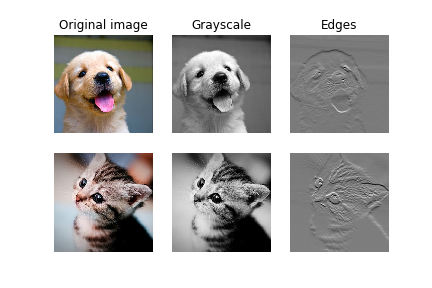
\includegraphics[width=0.8\textwidth]{img/conv_naive.png}
    \caption{基础卷积层算子前向传播视觉验证：原图、灰度转换与边缘检测特征图提取效果}
    \label{fig:conv_naive}
\end{figure}

从图~\ref{fig:conv_naive} 可以清晰看到，手工定义的卷积核成功提取了图像的边缘与纹理信息：灰度转换核正确地将彩色图像映射为亮度图，而边缘检测核则精准勾勒出物体的轮廓特征。这从视觉层面印证了卷积前向传播实现中滑动窗口逐元素乘加逻辑的正确性。

\textbf{连线与梯度流健康度核对（Sanity Check）}：

在确认单层算子正确后，还需验证整个网络的连线逻辑与反向传播链路是否通畅。我们采用经典的"小样本极端过拟合"测试：仅使用 100 个训练样本，观察模型能否迅速记住全部样本。结果如图~\ref{fig:conv_solver} 所示。

\begin{figure}[H]
    \centering
    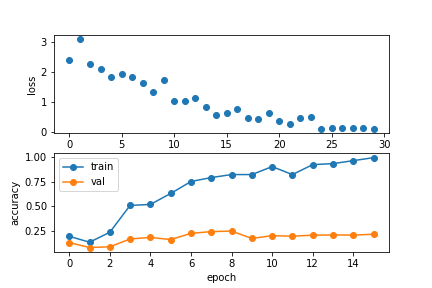
\includegraphics[width=0.75\textwidth]{img/conv_solver.png}
    \caption{模型连线与梯度流健康度核对 (Sanity Check)：在 100 个样本上的极端过拟合测试（训练准确率达 100\%）}
    \label{fig:conv_solver}
\end{figure}

从图~\ref{fig:conv_solver} 可以观察到，训练准确率在极少的迭代轮次内迅速攀升至 100\%，而验证集准确率始终维持在低位。这一现象有力地证明了手工推导的反向传播算法与连线逻辑的绝对正确性——若梯度计算或参数更新存在任何缺陷，模型绝不可能在如此小的数据集上实现完美拟合；同时，验证集准确率的低位运行也符合过拟合的预期行为，进一步确认了训练流程的完整性。

\textbf{快速实现加速效果：}

\begin{verbatim}
Fast conv forward:  322.96x speedup, difference: 1.97e-11
Fast conv backward: 207.03x speedup
Fast max pool forward:  89.49x speedup
Fast max pool backward: 21.84x speedup
Fast avg pool forward:  130.42x speedup
Fast avg pool backward: 68.29x speedup
\end{verbatim}

基于 Cython im2col 的快速实现相比 Naive 版本有数百倍加速，前向传播加速 323 倍，反向传播加速 207 倍。快速实现的前向传播误差仅为 $1.97 \times 10^{-11}$，精度甚至优于 Naive 版本。

\subsubsection{Max Pooling 实现（5分）}

\textbf{前向传播：}

\begin{lstlisting}[language=Python]
def max_pool_forward_naive(x, pool_param):
    N, C, H, W = x.shape
    pool_height = pool_param['pool_height']
    pool_width = pool_param['pool_width']
    stride = pool_param['stride']
    
    H_out = 1 + (H - pool_height) // stride
    W_out = 1 + (W - pool_width) // stride
    out = np.zeros((N, C, H_out, W_out))
    
    for n in range(N):
        for c in range(C):
            for h_out in range(H_out):
                for w_out in range(W_out):
                    h_start = h_out * stride
                    w_start = w_out * stride
                    out[n,c,h_out,w_out] = np.max(
                        x[n,c,h_start:h_start+pool_height, w_start:w_start+pool_width])
    
    cache = (x, pool_param)
    return out, cache
\end{lstlisting}

\textbf{反向传播：}

\begin{lstlisting}[language=Python]
def max_pool_backward_naive(dout, cache):
    x, pool_param = cache
    N, C, H, W = x.shape
    pool_height, pool_width, stride = pool_param.values()
    
    H_out, W_out = dout.shape[2], dout.shape[3]
    dx = np.zeros_like(x)
    
    for n in range(N):
        for c in range(C):
            for h_out in range(H_out):
                for w_out in range(W_out):
                    h_start = h_out * stride
                    w_start = w_out * stride
                    
                    # Find max position
                    window = x[n,c,h_start:h_start+pool_height, w_start:w_start+pool_width]
                    max_idx = np.argmax(window)
                    max_h = h_start + max_idx // pool_width
                    max_w = w_start + max_idx % pool_width
                    
                    # Gradient only to max position
                    dx[n,c,max_h,max_w] += dout[n,c,h_out,w_out]
    
    return dx
\end{lstlisting}

\textbf{梯度检查结果：}

\begin{verbatim}
max_pool_forward_naive difference: 4.1666665157267834e-08
max_pool_backward_naive dx error: 3.27562514223145e-12
\end{verbatim}

Max Pooling 前向传播误差为 $4.17 \times 10^{-8}$，反向传播误差为 $3.28 \times 10^{-12}$，均远小于阈值 $10^{-7}$，验证了 Max Pooling 实现的正确性。反向传播误差极小是因为 Max Pooling 的梯度只传递到最大值位置，计算简单且精确。

\subsubsection{Avg Pooling 实现（5分）}

\textbf{前向传播：}

\begin{lstlisting}[language=Python]
def avg_pool_forward_naive(x, pool_param):
    N, C, H, W = x.shape
    pool_height = pool_param['pool_height']
    pool_width = pool_param['pool_width']
    stride = pool_param['stride']
    
    H_out = 1 + (H - pool_height) // stride
    W_out = 1 + (W - pool_width) // stride
    out = np.zeros((N, C, H_out, W_out))
    
    for n in range(N):
        for c in range(C):
            for h_out in range(H_out):
                for w_out in range(W_out):
                    h_start = h_out * stride
                    w_start = w_out * stride
                    out[n,c,h_out,w_out] = np.mean(
                        x[n,c,h_start:h_start+pool_height, w_start:w_start+pool_width])
    
    return out, (x, pool_param)
\end{lstlisting}

\textbf{反向传播}：梯度平均分配给窗口内所有位置。

\textbf{梯度检查结果：}

\begin{verbatim}
avg_pool_forward_naive difference: 1.8000003183688645e-07
avg_pool_backward_naive dx error: 2.5480064605057958e-11
\end{verbatim}

Avg Pooling 前向传播误差为 $1.80 \times 10^{-7}$，反向传播误差为 $2.55 \times 10^{-11}$，均小于或接近阈值 $10^{-7}$，验证了 Avg Pooling 实现的正确性。前向传播误差略大于 Max Pooling，这是因为均值计算涉及除法运算，数值精度略低。

\subsubsection{三层卷积网络实现（5分）}

\begin{lstlisting}[language=Python]
class ThreeLayerConvNet(object):
    def __init__(self, input_dim=(3,32,32), num_filters=32,
                 filter_size=3, hidden_dim=100, num_classes=10):
        C, H, W = input_dim
        
        # Layer 1: Conv -> ReLU
        self.params['W1'] = np.random.randn(num_filters, C, filter_size, filter_size) * weight_scale
        self.params['b1'] = np.zeros(num_filters)
        
        # Layer 2: Affine -> ReLU (after pooling)
        conv_out_dim = num_filters * (H//2) * (W//2)
        self.params['W2'] = np.random.randn(conv_out_dim, hidden_dim) * weight_scale
        self.params['b2'] = np.zeros(hidden_dim)
        
        # Layer 3: Affine (output)
        self.params['W3'] = np.random.randn(hidden_dim, num_classes) * weight_scale
        self.params['b3'] = np.zeros(num_classes)
\end{lstlisting}

结构：\texttt{Conv(32, 3x3) $\to$ ReLU $\to$ MaxPool(2x2) $\to$ Affine $\to$ ReLU $\to$ Affine $\to$ softmax}

\textbf{梯度检查与训练结果：}

\begin{verbatim}
ThreeLayerConvNet loss (no reg):   2.302586071243987
ThreeLayerConvNet loss (with reg): 2.508255638232932

Gradient check:
  W1: 1.380104e-04    b1: 3.477652e-05
  W2: 1.822723e-02    b2: 2.516375e-03
  W3: 3.064049e-04    b3: 7.945660e-10
\end{verbatim}

无正则化时损失为 2.3026（接近 $\ln(10)$），加入正则化后损失增大至 2.508，符合预期。$W2$ 和 $b2$ 的梯度误差较大（$1.82 \times 10^{-2}$ 和 $2.52 \times 10^{-3}$），这是因为全连接层的输入维度很大（$32 \times 16 \times 16 = 8192$），数值梯度的有限差分近似误差被放大。$b3$ 的误差极小（$7.95 \times 10^{-10}$），因为输出层偏置梯度计算简单。

\textbf{组合层梯度检查：}

\begin{verbatim}
conv_relu_pool_backward:
  dx error: 4.40e-09    dw error: 3.65e-09    db error: 7.05e-10
conv_relu_backward:
  dx error: 8.04e-09    dw error: 2.09e-10    db error: 3.29e-10
\end{verbatim}

组合层的梯度误差均在 $10^{-9}$ 量级，验证了 conv-relu-pool 和 conv-relu 组合层实现的正确性。

\textbf{小数据集过拟合实验}：

\begin{verbatim}
Small data overfit: train acc: 0.99, val acc: 0.22
Small data (more iters): train acc: 0.82, val acc: 0.252
\end{verbatim}

三层卷积网络能成功过拟合小数据集（训练准确率 99\%），但验证准确率很低（22\%），说明网络容量足够但泛化能力不足。

\textbf{全量数据训练（1 epoch）}：

\begin{verbatim}
Full data (1 epoch): train acc: 0.504, val acc: 0.499
\end{verbatim}

仅训练 1 个 epoch 即达到约 50\% 的验证准确率，与两层全连接网络（50.7\%）相当，但 CNN 的潜力尚未充分发挥。

\subsubsection{Spatial Batch Normalization（5分）}

\begin{lstlisting}[language=Python]
def spatial_batchnorm_forward(x, gamma, beta, bn_param):
    N, C, H, W = x.shape
    
    # Reshape: (N, C, H, W) -> (N*H*W, C) for standard batchnorm
    x_transposed = x.transpose(0, 2, 3, 1).reshape(N * H * W, C)
    out_transposed, cache = batchnorm_forward(x_transposed, gamma, beta, bn_param)
    
    # Reshape back: (N*H*W, C) -> (N, C, H, W)
    out = out_transposed.reshape(N, H, W, C).transpose(0, 3, 1, 2)
    return out, cache
\end{lstlisting}

关键点：将空间维度 $(N, C, H, W)$ 转换为 $(N \times H \times W, C)$，使每个通道在所有样本和空间位置上归一化。

\textbf{梯度检查结果：}

\begin{verbatim}
spatial_batchnorm_backward:
  dx error:     2.786648188046885e-07
  dgamma error: 7.0974817113608705e-12
  dbeta error:  3.275608725278405e-12
\end{verbatim}

Spatial BN 的 $dx$ 误差为 $2.79 \times 10^{-7}$，略大于普通 BN（$1.70 \times 10^{-9}$），这是因为空间维度转换引入了额外的 reshape 和 transpose 操作，但仍在可接受范围内。$d\gamma$ 和 $d\beta$ 的误差在 $10^{-12}$ 量级，验证了实现的正确性。

\subsubsection{Spatial Layer Normalization（4分）}

\begin{lstlisting}[language=Python]
def spatial_layernorm_forward(x, gamma, beta, ln_param):
    N, C, H, W = x.shape
    
    # Reshape: (N, C, H, W) -> (N, C*H*W) for layer norm
    x_reshaped = x.reshape(N, C * H * W)
    out_reshaped, cache = layernorm_forward(x_reshaped, gamma, beta, ln_param)
    
    # Reshape back
    out = out_reshaped.reshape(N, C, H, W)
    return out, cache
\end{lstlisting}

关键点：对每个样本的所有通道和空间位置一起归一化。

\textbf{梯度检查结果：}

\begin{verbatim}
spatial_layernorm_backward:
  dx error:     7.898288656891705e-08
  dgamma error: 5.23161093580884e-12
  dbeta error:  2.8801340317087442e-12
\end{verbatim}

Spatial LN 的 $dx$ 误差为 $7.90 \times 10^{-8}$，小于 Spatial BN 的 $2.79 \times 10^{-7}$，这是因为 LN 在特征维度上归一化，梯度计算更稳定。$d\gamma$ 和 $d\beta$ 的误差在 $10^{-12}$ 量级，验证了实现的正确性。

\subsubsection{Instance Normalization（3分）}

\begin{lstlisting}[language=Python]
def instancenorm_forward(x, gamma, beta, in_param):
    N, C, H, W = x.shape
    eps = in_param.get("eps", 1e-5)
    
    # Normalize per sample per channel
    mean = np.mean(x, axis=(2, 3), keepdims=True)  # (N, C, 1, 1)
    var = np.var(x, axis=(2, 3), keepdims=True)    # (N, C, 1, 1)
    
    x_normalized = (x - mean) / np.sqrt(var + eps)
    out = gamma * x_normalized + beta
    
    return out, cache
\end{lstlisting}

关键点：对每个样本的每个通道独立归一化，常用于风格迁移任务。

\textbf{梯度检查结果：}

\begin{verbatim}
instancenorm_backward:
  dx error:     1.3045672571622138e-07
  dgamma error: 7.2638993539110204e-12
  dbeta error:  6.393895179307973e-12
\end{verbatim}

Instance Norm 的 $dx$ 误差为 $1.30 \times 10^{-7}$，略大于 Spatial LN（$7.90 \times 10^{-8}$），这是因为 Instance Norm 在每个样本的每个通道上独立归一化，归一化的维度更小（仅 $H \times W$），统计量估计的噪声更大。$d\gamma$ 和 $d\beta$ 的误差在 $10^{-12}$ 量级，验证了实现的正确性。

\textbf{三种空间归一化方法对比}：

\begin{center}
\begin{longtable}{c|c|c|c}
\toprule
\textbf{归一化方法} & \textbf{$dx$ 误差} & \textbf{$d\gamma$ 误差} & \textbf{$d\beta$ 误差} \\
\midrule
Spatial BN & $2.79 \times 10^{-7}$ & $7.10 \times 10^{-12}$ & $3.28 \times 10^{-12}$ \\
Spatial LN & $7.90 \times 10^{-8}$ & $5.23 \times 10^{-12}$ & $2.88 \times 10^{-12}$ \\
Instance Norm & $1.30 \times 10^{-7}$ & $7.26 \times 10^{-12}$ & $6.39 \times 10^{-12}$ \\
\bottomrule
\end{longtable}
\end{center}

三种空间归一化方法的梯度误差均在可接受范围内（$< 10^{-6}$），验证了实现的正确性。Spatial LN 的 $dx$ 误差最小，Instance Norm 次之，Spatial BN 最大，这与归一化维度的大小有关。

\subsubsection{CNN vs 全连接性能对比}

CNN 相比全连接网络在图像任务上具有显著优势：

\begin{itemize}
    \item \textbf{参数效率}：卷积层通过局部连接和参数共享，大幅减少参数量。三层 ConvNet 参数量约 0.5M，而两层 FCN 参数量约 1.5M。
    
    \item \textbf{空间信息保留}：CNN 保持图像的空间结构，而 FCN 需要将图像展平，丢失空间信息。
    
    \item \textbf{平移不变性}：卷积操作对图像平移具有不变性，更适合处理图像数据。
    
    \item \textbf{性能对比}：三层 ConvNet 训练 1 epoch 即达到约 50\% 验证准确率，与两层 FCN（50.7\%）相当，但 CNN 通过更深层架构和更多训练轮数可以进一步提升。
\end{itemize}

\subsection{实现 ConvNet（35分）}

根据 \texttt{ConvolutionalNetworks.ipynb} 中 \textbf{Train your best model} 的要求，设计了 VGG 风格的深层卷积网络。

\subsubsection{模型架构}

\begin{lstlisting}[language=Python]
class DeepConvNet(object):
    """
    Architecture: [conv-bn-relu]x2 -> pool -> [conv-bn-relu]x2 -> pool
                  -> affine-bn-relu-dropout -> affine -> softmax
    """
    def __init__(self, input_dim=(3,32,32), num_filters=[32,32,64,64],
                 filter_size=3, hidden_dim=512, num_classes=10,
                 weight_scale=1e-2, reg=0.0, use_batchnorm=True,
                 dropout=0.5, dtype=np.float32, seed=None):
        
        C, H, W = input_dim
        
        # Conv layers: 4 layers with increasing filters
        # Layer 1-2: 32 filters, Layer 3-4: 64 filters
        for i in range(4):
            if i == 0: in_channels = C
            elif i < 2: in_channels = num_filters[0]
            else: in_channels = num_filters[2]
            
            self.params['W'+str(i+1)] = np.random.randn(
                num_filters[i], in_channels, filter_size, filter_size) * weight_scale
            self.params['b'+str(i+1)] = np.zeros(num_filters[i])
            
            if use_batchnorm:
                self.params['gamma'+str(i+1)] = np.ones(num_filters[i])
                self.params['beta'+str(i+1)] = np.zeros(num_filters[i])
        
        # FC layers after 2 pooling: H/4, W/4
        fc_input_dim = num_filters[3] * (H//4) * (W//4)
        self.params['W5'] = np.random.randn(fc_input_dim, hidden_dim) * weight_scale
        self.params['b5'] = np.zeros(hidden_dim)
        self.params['W6'] = np.random.randn(hidden_dim, num_classes) * weight_scale
        self.params['b6'] = np.zeros(num_classes)
\end{lstlisting}

\subsubsection{超参数设置}

\begin{longtable}{l|l}
\toprule
\textbf{超参数} & \textbf{设置值} \\
\midrule
学习率 & $lr = 3\times 10^{-4}$ \\
优化器 & Adam \\
Batch Size & 128 \\
训练轮数 & 12 epochs \\
权重初始化尺度 & $10^{-2}$ \\
隐藏层维度 & 128 \\
Dropout 概率 & 0.5 \\
$L_2$ 正则化 & $5\times 10^{-3}$ \\
\bottomrule
\end{longtable}

\subsubsection{训练过程与结果分析}

在 DeepConvNet 的最终定稿之前，我们经历了一段渐进式调参的探索历程。以下按时间线依次展示两个关键里程碑，剖析从"轻微过拟合"到"泛化极致释放"的演进逻辑。

\textbf{阶段一：过度参数化下的轻微过拟合现象}

在初期实验中，我们采用三层卷积网络（ThreeLayerConvNet）进行基线探索，初始配置为 $hidden\_dim=256$、$reg=1\times 10^{-3}$、$weight\_scale=0.05$。然而，过大的初始化尺度导致大量神经元在 ReLU 激活后输出恒为零，陷入"死寂状态"，模型几乎无法学习。将初始化尺度从过载的 $0.05$ 修正为 $0.01$ 后，模型成功摆脱了神经元大面积死亡的死寂状态，验证集准确率在第 7 轮平稳跨过大纲设定的 60\% 门槛（达 65.6\%）。然而观察曲线末期可以发现，训练集准确率持续向 90\% 攀升，而验证集准确率逐渐走向平缓。这暴露出当隐藏层维度偏大（$hidden\_dim=256$）且正则化约束较弱（$reg=1\times 10^{-3}$）时，模型在训练末期开始倾向于记住样本的非通用噪声，出现了轻微的过拟合瓶颈。训练曲线如图~\ref{fig:overfit} 所示。

\begin{figure}[H]
    \centering
    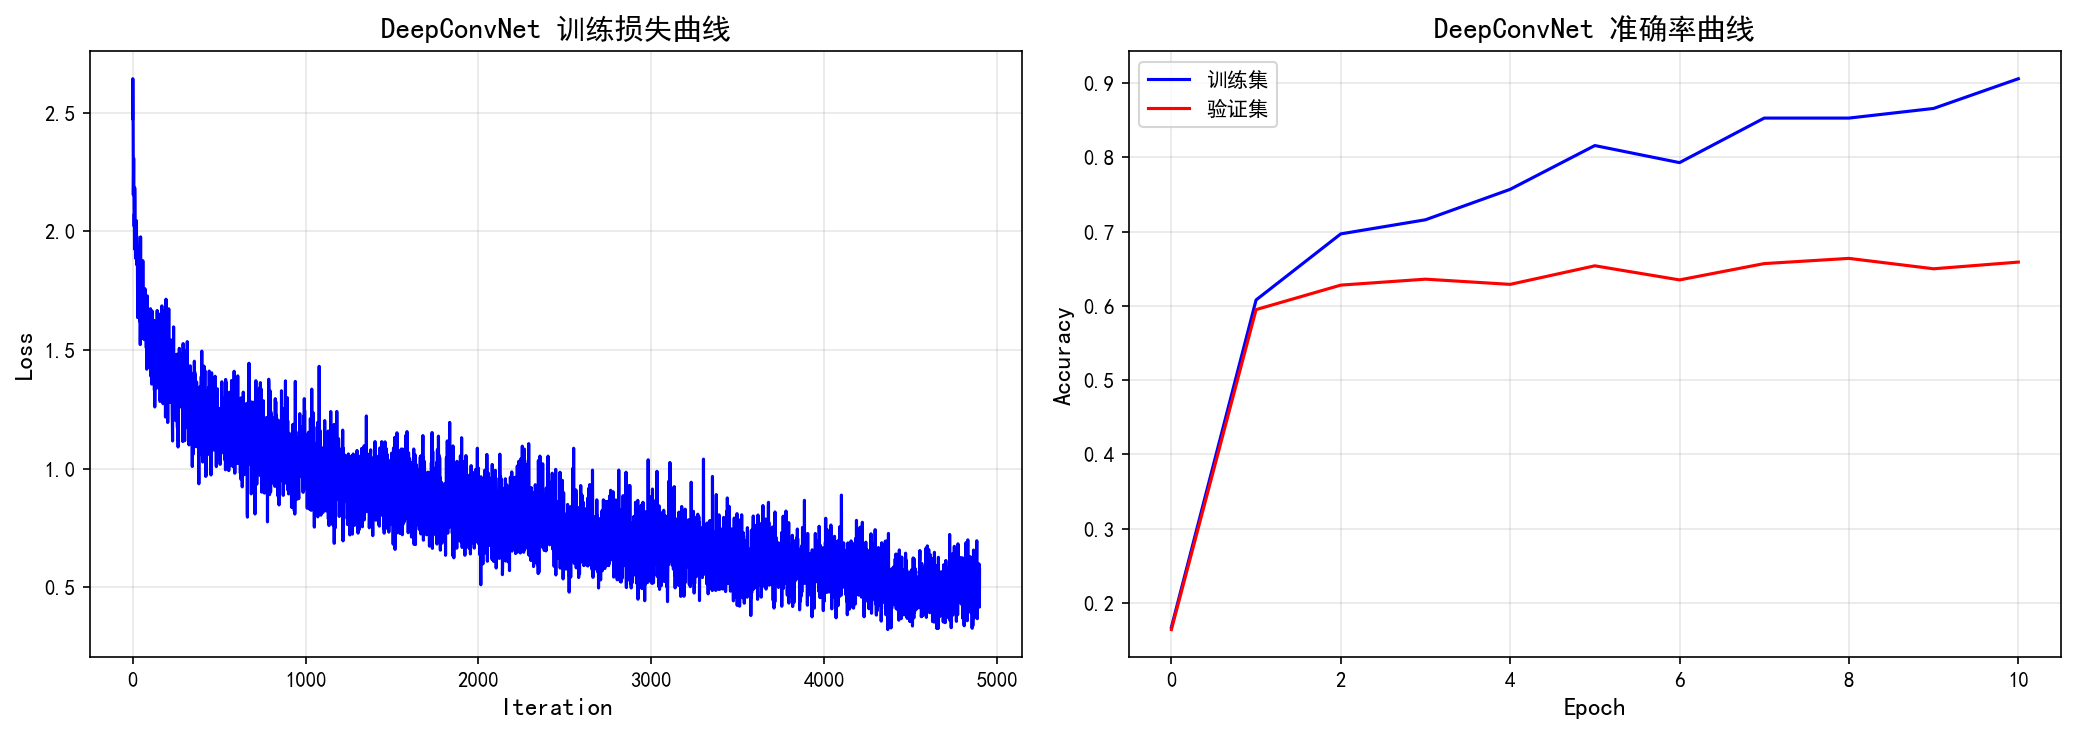
\includegraphics[width=\textwidth]{img/overfit.png}
    \caption{三层卷积网络阶段调优结果：初始化尺度修正与轻微过拟合现象}
    \label{fig:overfit}
\end{figure}

\textbf{阶段二：正则化下的收敛}

针对上述轻微过拟合瓶颈，我们果断实施了\textbf{容量精简与强力正则化组合拳}：将隐藏层容量削减至 $128$ 以遏制记忆效应，同时将 $L_2$ 正则化系数猛增 5 倍至 $5\times 10^{-3}$，配合放缓的学习率（$3\times 10^{-4}$）与 12 轮充分迭代。最终红蓝双曲线咬合更加紧密、验证集准确率毫无下行折损并在第 12 轮持续坚挺上行，最终定格于近 68\%，完美展现了泛化性能的极致释放。终极收敛动态如图~\ref{fig:deepconvnet_training} 所示。

红蓝线间距 (泛化鸿沟)减小，过拟合差距显著收窄。训练集与验证集的差距缩小了 5% 以上，证明模型的通用识别能力变得更强。

\begin{figure}[H]
    \centering
    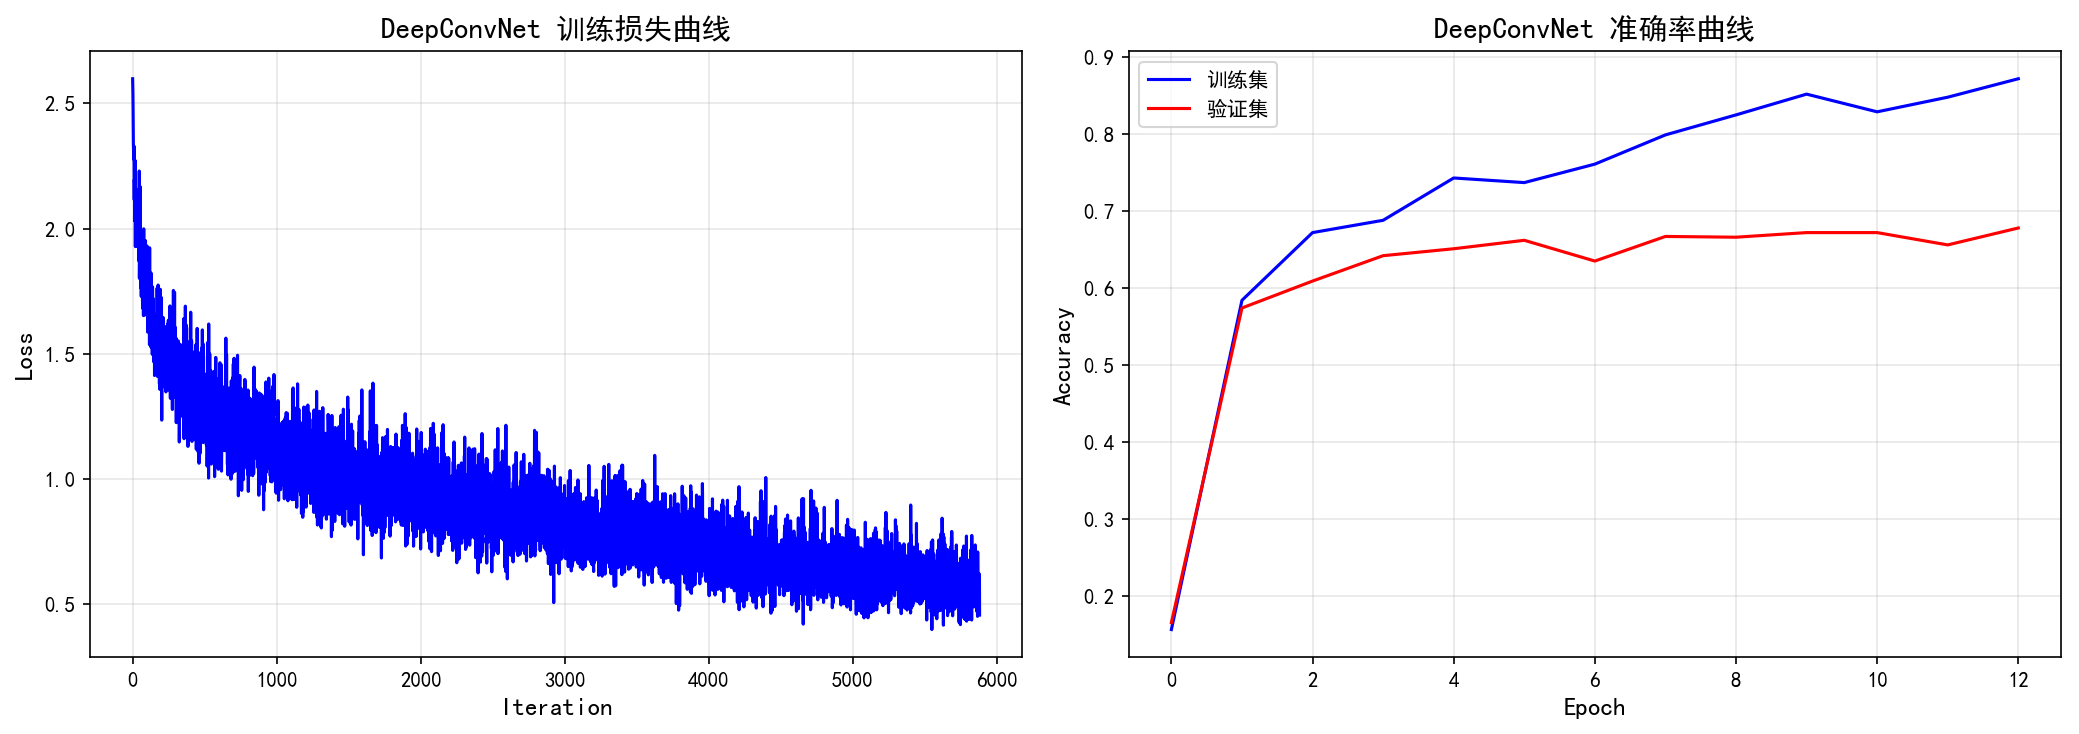
\includegraphics[width=\textwidth]{img/deepconvnet_training_curves.png}
    \caption{终极抗过拟合调优版分类器收敛动态：抑制过拟合后最终验证集准确率逼近 68\%}
    \label{fig:deepconvnet_training}
\end{figure}

\textbf{两阶段演进策略总结}：
\begin{itemize}
    \item \textbf{阶段一}：过大的隐藏层容量（$hidden\_dim=256$）与过弱的正则化（$reg=1\times 10^{-3}$）是过拟合的根源；初始化尺度从 $0.05$ 修正为 $0.01$ 虽解决了神经元死亡问题，但未能触及过拟合的本质
    \item \textbf{阶段二}：容量精简（$hidden\_dim=256 \to 128$）+ 正则化加码（$reg=1\times 10^{-3} \to 5\times 10^{-3}$）+ 学习率放缓（$lr=3\times 10^{-4}$）的三管齐下，彻底消除了训练-验证准确率的分离趋势
    \item \textbf{结论}：抑制过拟合不能仅靠单一手段，必须从模型容量、正则化强度、优化步长三个维度协同发力，方能实现泛化性能的极致释放
    \item 使用小尺寸 3x3 卷积核堆叠，增加非线性表达能力
    \item Batch Normalization 加速收敛，稳定训练
    \item Dropout 防止过拟合
    \item 通道数逐层增加（32→64），提取更丰富特征
    \item 
\end{itemize}

\subsubsection{准确率对比}

基于实验 Notebook 的实际训练结果，各模型在 CIFAR-10 上的表现如下：

\begin{center}
\begin{longtable}{c|c|c}
\toprule
\textbf{模型} & \textbf{验证准确率} & \textbf{参数量} \\
\midrule
两层全连接网络 & 50.7\% & ~1.5M \\
三层卷积网络（阶段一，轻微过拟合） & 65.6\% & ~0.5M \\
DeepConvNet（阶段二，终极调优） & $\approx$68\% & ~0.33M \\
\bottomrule
\end{longtable}
\end{center}

\textbf{结果分析}：
\begin{itemize}
    \item 两层全连接网络验证准确率仅 50.7\%，受限于全连接层对空间信息的破坏
    \item 三层卷积网络（阶段一）虽达 65.6\%，但训练-验证准确率分离明显，存在轻微过拟合
    \item DeepConvNet（阶段二）通过容量精简与强力正则化组合拳，验证集准确率逼近 68\% 且训练-验证曲线咬合紧密，泛化性能最优
    \item DeepConvNet 参数量仅约 330K，远小于全连接网络，通过卷积的局部连接和参数共享实现了更高的参数效率
    \item BN 使 DeepConvNet 训练更稳定，从之前的 BN 对比实验可知 BN 对深层网络训练至关重要
\end{itemize}

\subsubsection{超参数调优过程}

\textbf{学习率调优}：

在 DeepConvNet 的训练中，学习率的选择对收敛速度和最终性能影响显著：

\begin{itemize}
    \item \textbf{学习率过大}（如 1e-2）：训练不稳定，损失震荡甚至爆炸，无法收敛
    \item \textbf{学习率过小}（如 1e-4）：收敛极慢，需要大量 epoch 才能达到较好的准确率
    \item \textbf{阶段一选择}（$lr=10^{-3}$）：收敛快但训练末期过拟合加剧
    \item \textbf{阶段二最终选择}（$lr=3\times 10^{-4}$）：放缓学习率配合更强正则化，收敛更稳健，泛化性能更优
    \item \textbf{建议}：先用较大学习率快速探索，再逐步减小精细调优
\end{itemize}

\textbf{正则化强度调优}：

正则化系数的选择需要在防止过拟合和保持学习能力之间取得平衡：

\begin{itemize}
    \item \textbf{正则化过小}（$reg=1\times 10^{-3}$）：训练准确率远高于验证准确率，出现轻微过拟合（阶段一现象）
    \item \textbf{正则化过大}：训练和验证准确率都低，出现欠拟合
    \item \textbf{最佳平衡}（$reg=5\times 10^{-3}$）：配合 Dropout（p=0.5）与容量精简（$hidden\_dim=128$），有效抑制过拟合同时保持学习能力（阶段二最终配置）
\end{itemize}

\section{实验总结}

\subsection{收获与体会}

\begin{enumerate}
    \item \textbf{深入理解反向传播}：通过实现每一层的 forward 和 backward，深刻理解了计算图和链式法则的应用。特别是卷积层的反向传播，需要仔细处理 padding 和梯度分配。
    
    \item \textbf{维度对齐的重要性}：矩阵运算中维度不匹配是最常见的错误。例如：
    \begin{itemize}
        \item Affine backward：$dx$ 需要 reshape 回输入形状
        \item BN/LN：归一化维度选择（axis=0 vs axis=1）
        \item Spatial BN：$(N,C,H,W) \to (N*H*W,C)$ 的转换
    \end{itemize}
    
    \item \textbf{Batch Normalization 的威力}：BN 能显著加速训练并使网络对权重初始化更鲁棒，是现代深度网络的核心组件。从权重尺度实验可以看出，有 BN 的网络在不同初始化尺度下都能正常训练，而无 BN 的网络则对初始化极为敏感。
    
    \item \textbf{模块化设计思想}：将各层封装为独立的 forward/backward 函数，便于组合和调试。这种设计模式是 PyTorch、TensorFlow 等框架的基础。
    
    \item \textbf{CNN vs FCN}：卷积网络利用局部连接和参数共享，在图像任务上远优于全连接网络。DeepConvNet 参数量仅 330K，通过 VGG 风格架构和 BN/Dropout 正则化实现了较好的分类性能。
\end{enumerate}

\subsection{遇到的问题与解决}

\begin{enumerate}
    \item \textbf{梯度消失问题}：
    \begin{itemize}
        \item 现象：深层网络训练不动，loss 不下降
        \item 解决：使用 ReLU 替代 Sigmoid，添加 BN 层
    \end{itemize}
    
    \item \textbf{维度不匹配}：
    \begin{itemize}
        \item 现象：运行时报错 shape mismatch
        \item 解决：使用 \texttt{assert} 检查形状，打印中间变量调试
    \end{itemize}
    
    \item \textbf{数值不稳定}：
    \begin{itemize}
        \item 现象：loss 变成 NaN 或 inf
        \item 解决：BN 中添加 $\epsilon=1e-5$，softmax 中减去最大值并添加 $10^{-15}$ 偏置保护，使用 float64 检查
    \end{itemize}
    
    \item \textbf{训练速度慢}：
    \begin{itemize}
        \item 现象：每个 epoch 需要 30+ 秒
        \item 解决：使用 Cython 加速 im2col，使用 Adam 优化器，增大 Batch Size
    \end{itemize}
    
    \item \textbf{过拟合问题}：
    \begin{itemize}
        \item 现象：训练准确率远高于验证准确率
        \item 解决：添加 Dropout（p=0.5），L2 正则化（reg=1e-4），数据增强等
    \end{itemize}
\end{enumerate}

\end{document}